This chapter presents our reference plane assisted sketching
interface for progressive shape design. The underlying algorithms
that support and implement the sketching interface are also
provided.

%-------------------------------------------------------------------------
\section{Introduction}
\label{ch3:sec:intro}

%Traditional modeling methods & sketch-based modeling
%Creating and editing 3D models is a fundamental task in geometric modeling and computer graphics. Meanwhile it is also a tedious process with current 3D modeling packages such as Maya, 3DS Max and SolidWorks, which use the WIMP-style (Windows, Icon, Menu, Pointer) interfaces to construct and manipulate 3D models in a highly careful and skillful manner. The process and interactions in these packages are far from designers or artists' habits and environments. Sketch-based modeling allows users to do modeling by sketching 2D strokes, which thus provides a new way for 3D modeling. It is suitable for early conceptual design and idea communication.

%What is sketch-based modeling, main techniques
It has been introduced in previous chapters that sketch-based
modeling allows the user to do 3D modeling by sketching 2D strokes,
which provides a convenient and intuitive way over the traditional
modeling packages using the WIMP-style (Windows, Icon, Menu,
Pointer) interfaces. Sketch-based modeling typically uses freeform
curves (or strokes) as the basic modeling metaphor and allows user
to produce 3D models using sketching or sculpting methods, which are
quite similar to the creation behavior of artists in reality. In the
sketching method, the user draws the 2D contours of a desired shape
from scratch and the corresponding 3D model will be automatically
generated after the sketching; while in the sculpting method, the
user starts the creation from a very rough shape and uses various
sketches or gestures to carve, deform, extend or smooth it to a
desired one.

%the problems of sketch-based modeling.
%problem 1: no hint/reference shapes in sketching, sketches not preserved in sculpting
Note that the distinguished features of sketch-based modeling also
propose some challenges. One challenge comes from the process of the
sketching and sculpting operations. Since the sketching operation
does not directly communicate about the shape that the user has in
his mind, without the help of visual mediums for describing the 3D
shape during drawings, sketching a model from scratch takes a great
deal of skill~\cite{CIW08}. However, it is not easy to design an
intuitive sketching interface and develop the supporting modeling
algorithm to give the user necessary visual hints for the sketching
operation. As introduced in Section~\ref{ch2:sec:sbim:sketch},
existing sketching methods are designed to generate the result model
after all the curves have been sketched, ambiguities may exist on
both the perception on the input sketches and output shape. Although
the sculpting operation provides an alternative solution for
intuitive 3D modeling by allowing the iterative carve operation from
a rough shape, it will be tedious when the shape to create is not
simple and the quality of the model may not be well preserved after
many editing operations. Meanwhile, with the progress of sculpting,
previous sketches which represent the user's intentions on
describing the shape of the model may probably be changed or
discarded.


%problem 2: 2D sketch --> 3D model
Another challenge is that when doing 3D modeling, we have to find
indirect ways to interact with the 3D space using the input devices
operating on the 2D computer screen. A classical solution to this
problem is to use the Arcball~\cite{SK92} when we view a 3D object
in a virtual environment. As for the 3D modeling tasks, this problem
will become tougher for novice users who are not familiar or
sensitive with the 3D space. It is very difficult, if not
impossible, to specify the 3D position and orientation when
sketching strokes into free space, without the help of references.

%problem 3: lack of stroke rules
Last but not least, although there have been  some general rules on
perceiving the user sketches of depicting 3D shapes~\cite{HD00}, it
remains difficult to interpret and map the strokes that the user
sketches for specific modeling tasks. Proper interpretation of
sketching is very important because it is related to whether the
system correctly understands the user's intention and whether the
creation and editing is successfully performed.

%our contributions
In this chapter, we propose methods to solve  these problems. First,
to enhance the sketching function, we introduce a progressive
modeling approach which takes both the existing sketches and the
constructed 3D shape as references, when the user creates a 3D model
through iterative sketching. In this way, the user will have a clear
mind of the 3D shape he/she has sketched and unexpected model shape
resulting from perception ambiguity can be avoided. Meanwhile, all
the sketches which represent the user's depiction of the 3D shape
are preserved.
%To better support this approach, we propose a new surface reconstruction algorithm which builds a 3D smooth surface with arbitrary topology from user sketched cross sections in real time. Comparing to existing algorithms, our method is able to produce natural shape changes during the progressive modeling process regardless of the input order of the sketches, and makes the final surface be composed of only one component in most cases.

Second, to reasonably map the 2D user sketches into 3D space and
make the location and orientation of strokes in 3D space meaningful
and intuitive, we provide some reference geometry, with reference to
which the strokes were sketched. In particular, besides the shape in
its current design stage, we also use some auxiliary planes as
reference geometry. The auxiliary planes are automatically
constructed based on the user's sketches or default settings, and
can be further adjusted manually if not satisfactory.

Third, to partially eliminate the ambiguity of  understanding the
user input sketches, we introduce some rules for regularizing and
interpreting them. These rules consider both the semantic meaning of
the sketched strokes and human psychology.

Finally, by integrating all these techniques, we present a novel
sketching interface for creating and editing 3D models. It is
demonstrated that with help of the reference shapes and planes,
sketch-based 3D modeling becomes more flexible and easier, thus
leading to a more enjoyable touch of the 3D space for users.

%organization of the paper
The rest of this chapter is organized as follows:
Section~\ref{ch3:sec:ui} describes our sketching interface. The
underlying algorithms that support and implement our sketching
interface are explained in Section~\ref{ch3:sec:algo}. The
experimental results and discussions are provided in
Section~\ref{ch3:sec:result}.

%%-------------------------------------------------------------------------
%\section{Previous work}
%\label{Sec:Review}
%
%In recent years, many works on sketch-based modeling have been proposed~\cite{OSSJ09}. As has been introduced in Section~\ref{ch3:sec:intro}, they can be divided into the sketching and sculpting methods.
%
%sketching technique, single view sketching + rules/templates for interpreting
%The sketching technique usually lets the user sketch the silhouettes and feature lines to depict the 3D shape and then constructs the model automatically. One method is to allow the user to complete a single complex sketch from a fixed viewpoint, interpret the sketches according to some rules to map the 2D curves or strokes into 3D space and then reconstruct the 3D model. For example, CrossSketch~\cite{ASN07} makes use of the Cubic Corners to reconstruct the depth of the vertices. It can generate an open surface with much details rather than a closed 3D mesh. The work~\cite{KPG05} interprets the 2D curve between each pair of intersection points as a 3D one with minimum normal curvature. A closed surface is then constructed from each surface patch bounded by the 3D curves. Masry and Lipson~\cite{ML07} present a system which is able to construct rigid 3D objects from both straight and cursive lines. The Maximum weight Spanning Tree (MST) is used to determine the 3D depth of endpoint vertices of straight lines and the curves in 3D space is calculated using the gradient steepest descent algorithm. Besides these rules, there are also some other methods trying to interpret the single view sketches according to the existing template information~\cite{CNXDK08,KSV09}. Despite these efforts, it remains difficult to eliminate the ambiguities when mapping the 2D sketch into 3D when it becomes complex.
%
%sketching technique, multi-view
%The other method used in the sketching technique is to allow the user to sketch the 3D outlines of a model from multiple viewpoints. Ilovesketch~\cite{BBS08}, for example, allows the user to sketch the 3D profile curves of the model to create, by using some predefined gestures to change the viewpoints on a multi-touch display, and the final model is constructed in a patch-by-patch manner similar to the methods in~\cite{KPG05,RSWCT07}. VolumeViewer~\cite{SLJGAGL09} lets the user sketch the cross sections along contours of medical image slices and used the surface reconstruction algorithm proposed in~\cite{LBDLJ08} to build the final surface from the sketches. These methods can only reconstruct the model after all the curves have been sketched, thus providing little hints of the 3D shape to the user during the sketching process. A. Rivers et al~\cite{RDI10} present a system that is similar to traditional modeling interface. The user sketches the silhouettes of a 3D object from three orthogonal views and the final model is computed using the visual hull method. Similar designs can be found in~\cite{FMKCHDJ03}. However for a model with multiple components and different depths, the silhouettes under one viewpoint requires much imagination for novice users. Meanwhile, when the topology of the model is complex, it is not easy to maintain the coherence and validity of the sketches from multiple viewpoints without any rules for regularization and interpretation.
%
%sculpting, how to create the initial shape
%Different from the sketching technique, the sculpting method usually lets the user create a rough shape initially and then use various modeling tools to sculpt to a desired shape iteratively. Many methods have been proposed to generate a high-quality smooth surface from a closed contour, with the surface representations of the models being triangular mesh~\cite{IMT99,IH03,KH06,NISA07,NPAI09}, implicit surface~\cite{KHR02,SWSJ05,BMSdV10} or subdivision surface~\cite{NKS09}.
%
%sculpting, deformation, point handle
%After the rough shape has been generated, the user can then use various tools to edit the model through interweaving sketches and viewpoint changes. The most popular editing tool is the deformation tool, by which the user can interactively deform the model surface through manipulating a handle on it, with the goal of obtaining a smooth surface which is as similar to the original one as possible.~\cite{NISA07,SCLARS04,SA07,SWS10} proposed to let the user drag a point on the surface along the direction parallel to the screen and then compute its position according to the position of the camera. The new positions of the part of the surface to deform is then computed according to the positional change of the handle point by solving an optimization problem. This approach can give real-time feedback to the user and is suitable for interactive editing, but it is not intuitive enough for confirming the direction of deformation in 3D space. Meanwhile, it does not fit for the case where multiple handle points are desired to be manipulated at the same time.
%
%sculpting, deformation, curve handle
%Instead of manipulating a point, Nealen et al~\cite{NSAC05} proposed to deform a mesh by changing the shape of a handle curve on the surface. First, a curve is drawn on the mesh to serve as the handle curve. Then the model is rotated manually to a proper angle and the deformed curve is drawn on the screen. The 3D position of the new curve could be calculated according to the current viewpoint. SilSketch~\cite{ZNA07} extends this idea by automatically detecting the handle curve which is a part of the silhouette of the model and corresponds to a user input stroke for the deformed handle curve. Similar method can also be found in~\cite{KSV09}. Since these methods rely on the 2D screen and lack references for mapping the 2D information into 3D, the handle curve and its deformed shape are limited to be planar, which seems not flexible enough for editing the 3D surface.
%
%sculpting, other functions
%There are also some other sculpting functions, such as merging several simple objects into a complex one~\cite{KHR02,SWSJ05,SS08}, extruding, cutting, smoothing~\cite{IMT99,NISA07,KHR02}, and sketching features~\cite{NSAC05,NISA07,OSSJ05,GZ08} on the surface. We refer the readers to an excellent survey paper~\cite{OSSJ09} for a broad overview of these editing functions. The sculpting technique requires iterative or even boring operations if the initial shape is far from desired. The user sketched curves which represent the outlines of the model may probably be distorted or even erased by the following modeling operations. Meanwhile, the quality of the final shape cannot be guaranteed if too much operations are implemented. Thus it is more suitable for further adjustment after the overall shape of the 3D model has been stylized.


%-------------------------------------------------------------------------
\section{User interface}
\label{ch3:sec:ui}

Our sketching interface provides both the sketching and sculpting
tools for the user to create and edit a 3D model. The former is used
for sketching the shape of the model progressively, and the latter,
which includes a series of editing functions such as deformation,
extrusion and so on, is used to refine or further modify the created
model. The output is a triangular mesh, which is a popular
representation for digital geometry.

\subsection{Sketching tool}
\label{Sec:UI:sketch}

\begin{figure*} [htbp]
  \centering
  \subfigure[]{
    \centering
    \label{fig:pig:a} %% label for first subfigure
    \begin{minipage}[b]{0.18\textwidth}
      \centering
      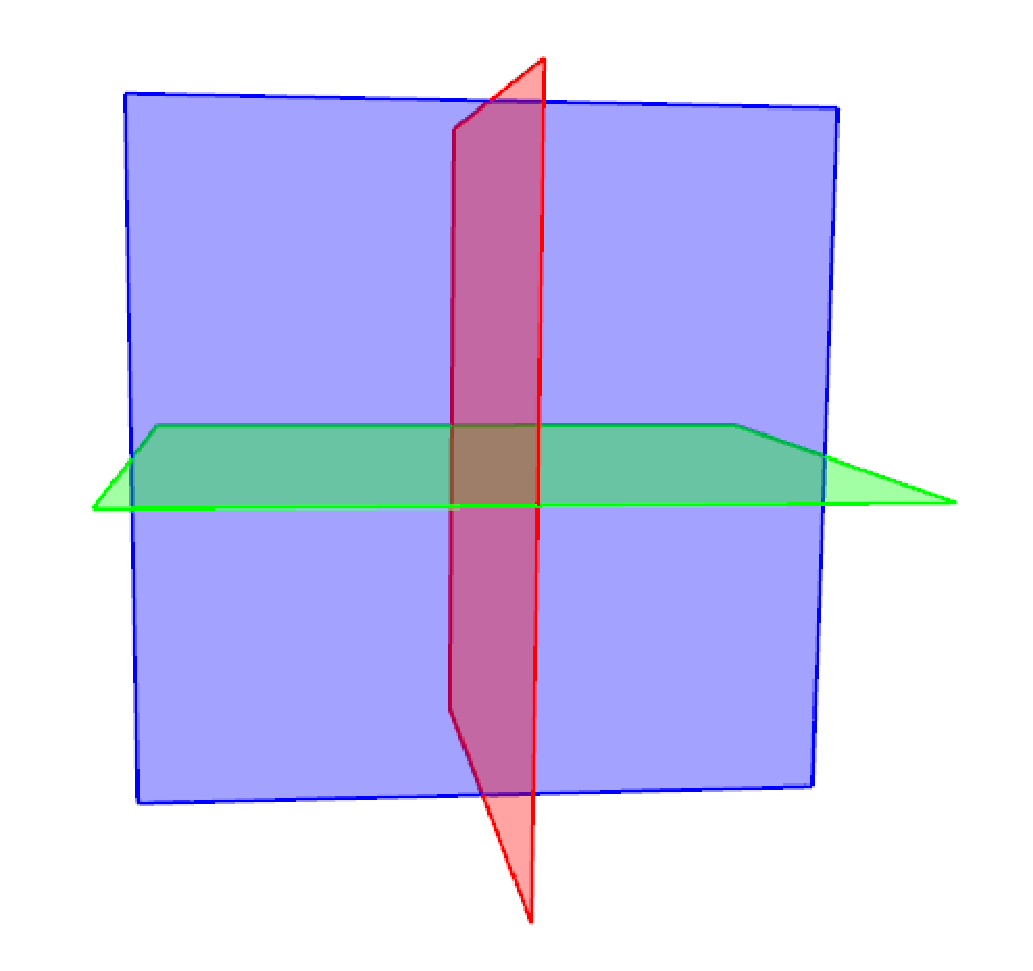
\includegraphics[scale=0.2]{figs/f3.pig-1.eps}
    \end{minipage}}
  \subfigure[]{
    \centering
    \label{fig:pig:b}
    \begin{minipage}[b]{0.18\textwidth}
      \centering
      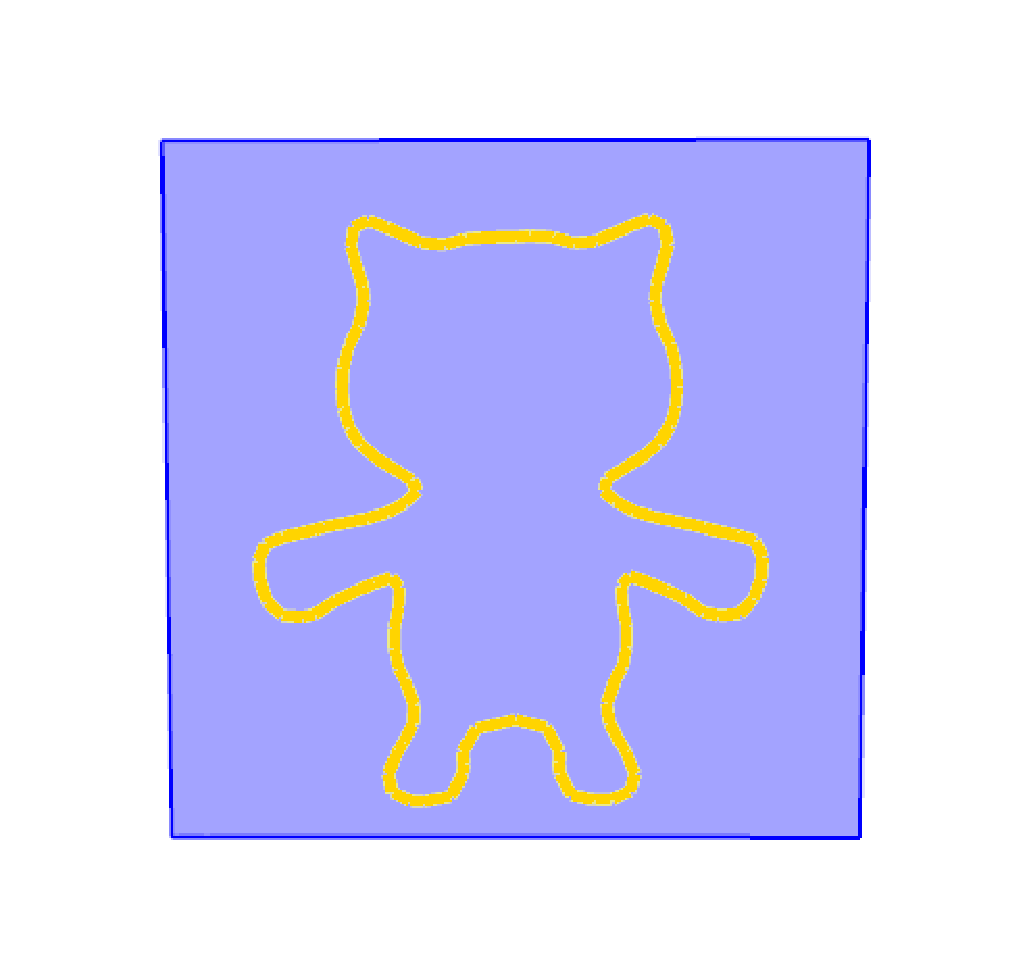
\includegraphics[scale=0.2]{figs/f3.pig-2.eps}
    \end{minipage}}
  \subfigure[]{
    \centering
    \label{fig:pig:c}
    \begin{minipage}[b]{0.18\textwidth}
      \centering
      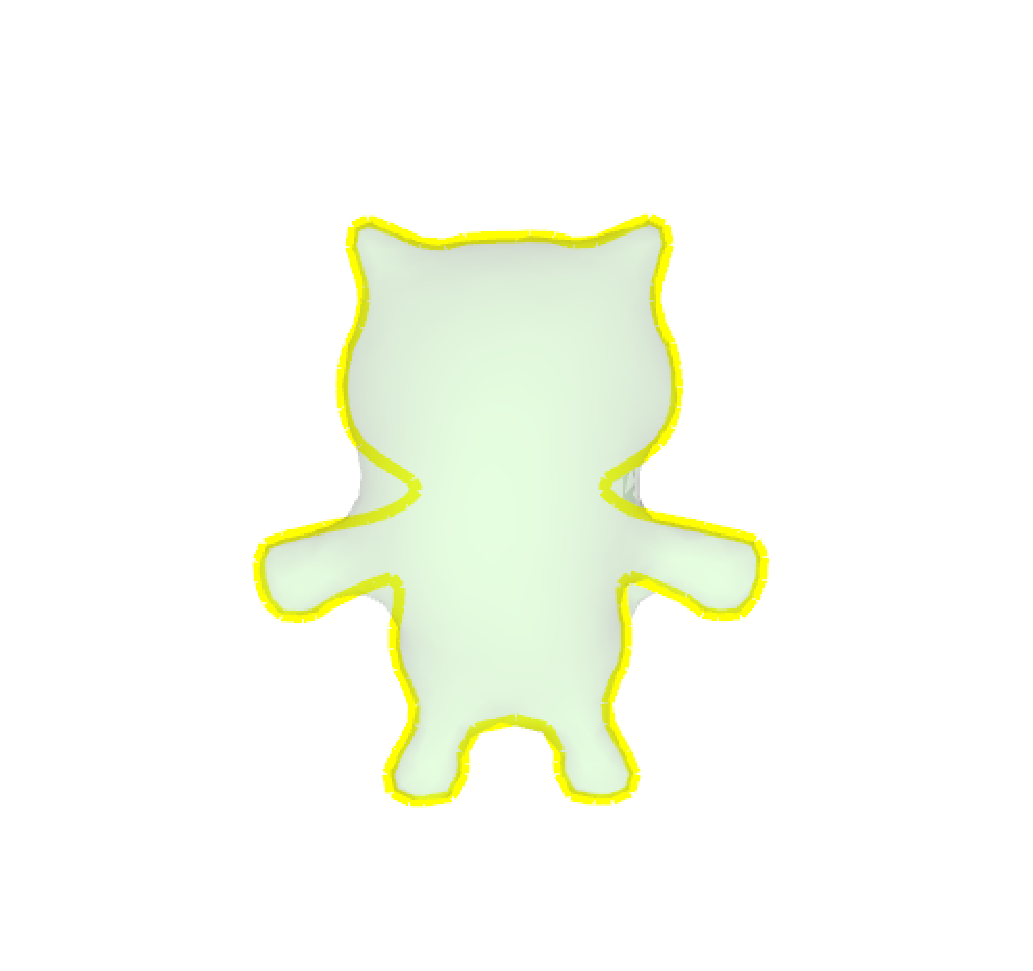
\includegraphics[scale=0.2]{figs/f3.pig-3.eps}
    \end{minipage}}
  \subfigure[]{
    \label{fig:pig:d}
    \begin{minipage}[b]{0.18\textwidth}
      \centering
      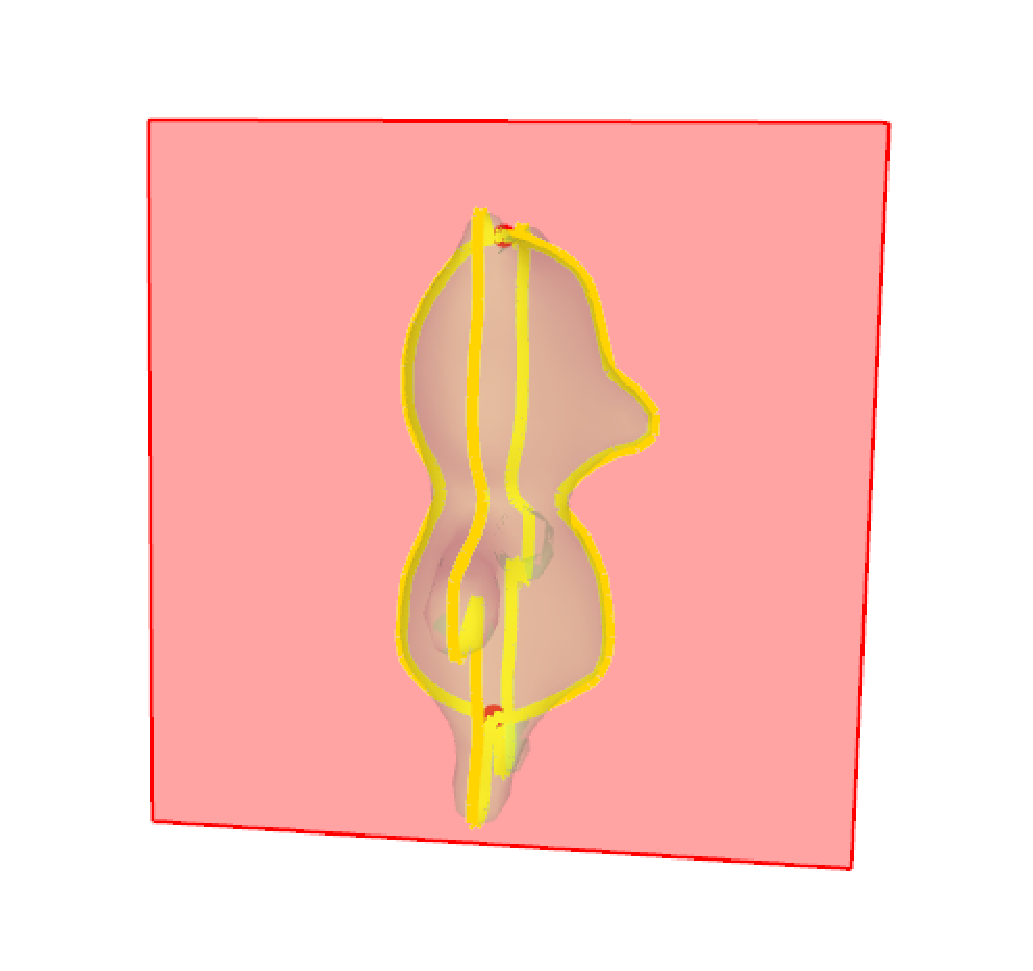
\includegraphics[scale=0.2]{figs/f3.pig-4.eps}
    \end{minipage}}
  \subfigure[]{
    \label{fig:pig:e}
    \begin{minipage}[b]{0.18\textwidth}
      \centering
      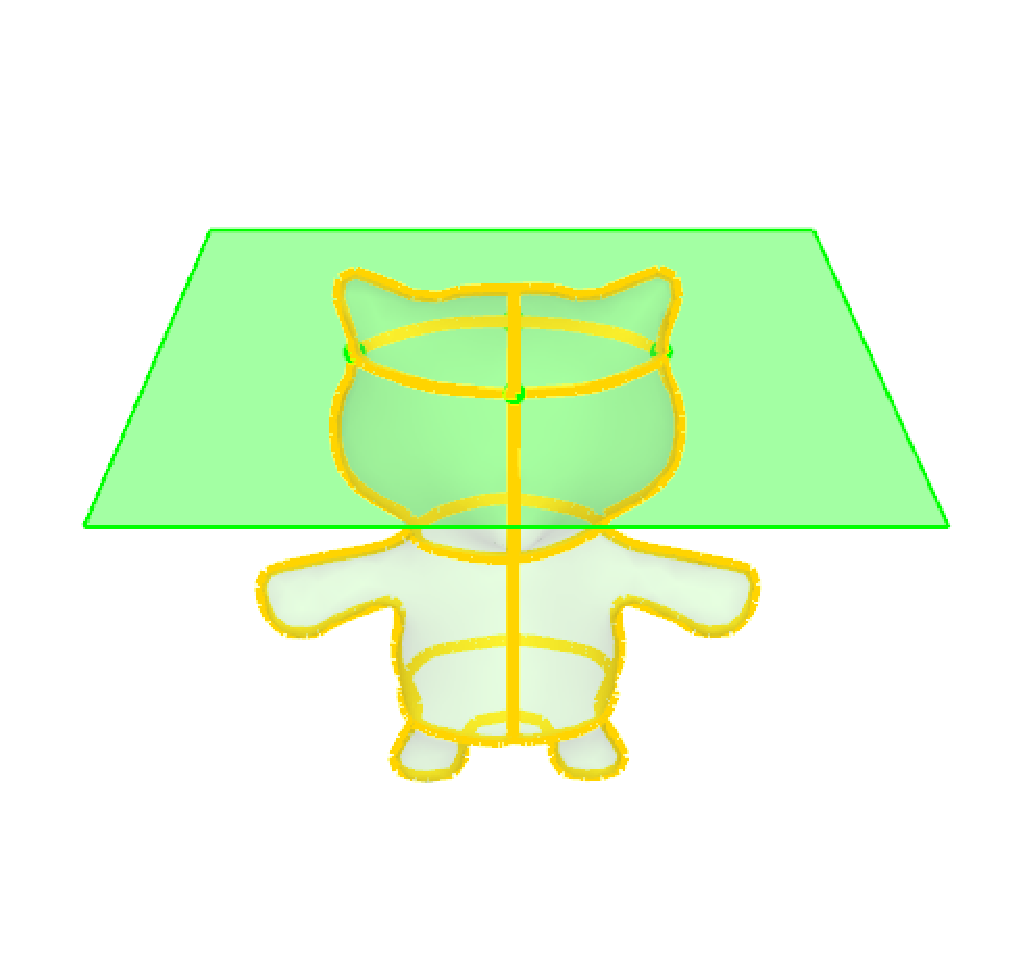
\includegraphics[scale=0.2]{figs/f3.pig-5.eps}
    \end{minipage}}
  \subfigure[]{
    \label{fig:pig:f}
    \begin{minipage}[b]{0.22\textwidth}
      \centering
      
\includegraphics[scale=0.22]{figs/f3.pig-6.eps}
    \end{minipage}}
  \subfigure[]{
    \label{fig:pig:g}
    \begin{minipage}[b]{0.22\textwidth}
      \centering
      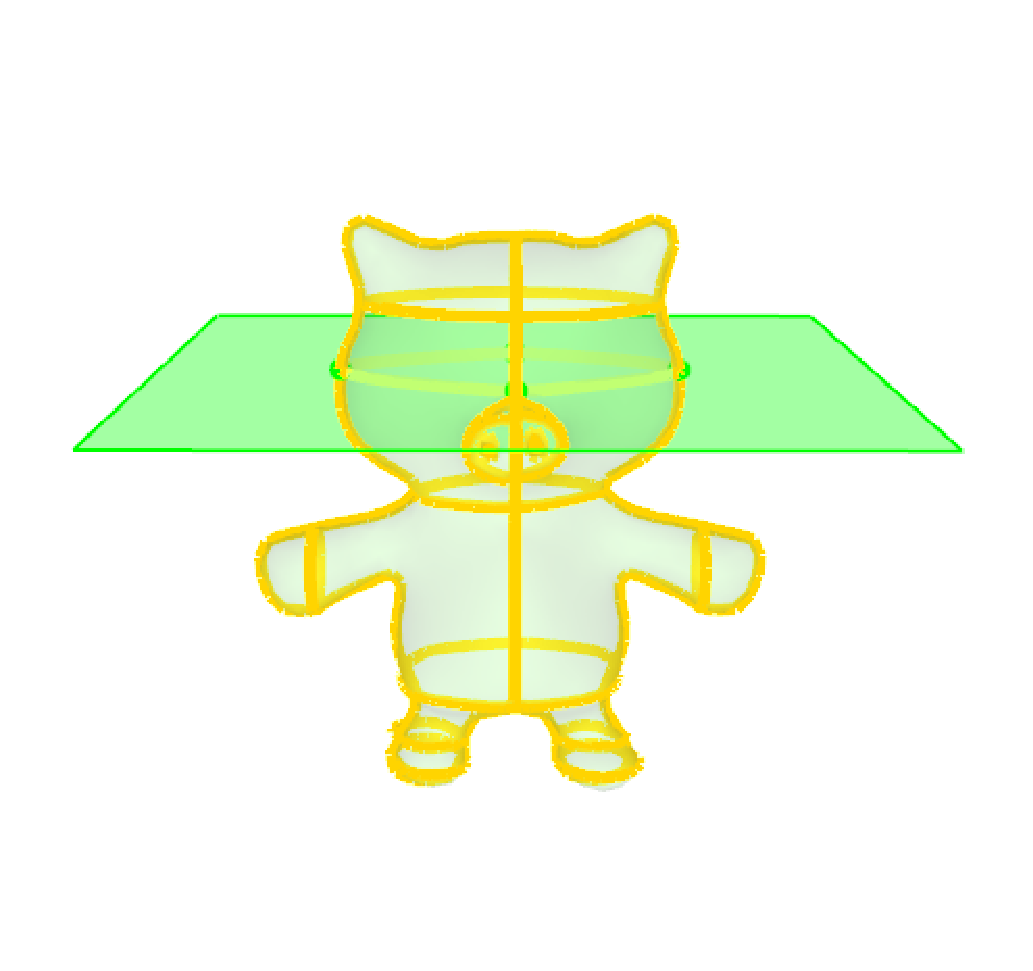
\includegraphics[scale=0.22]{figs/f3.pig-7.eps}
    \end{minipage}}
  \subfigure[]{
    \label{fig:pig:h}
    \begin{minipage}[b]{0.22\textwidth}
      \centering
      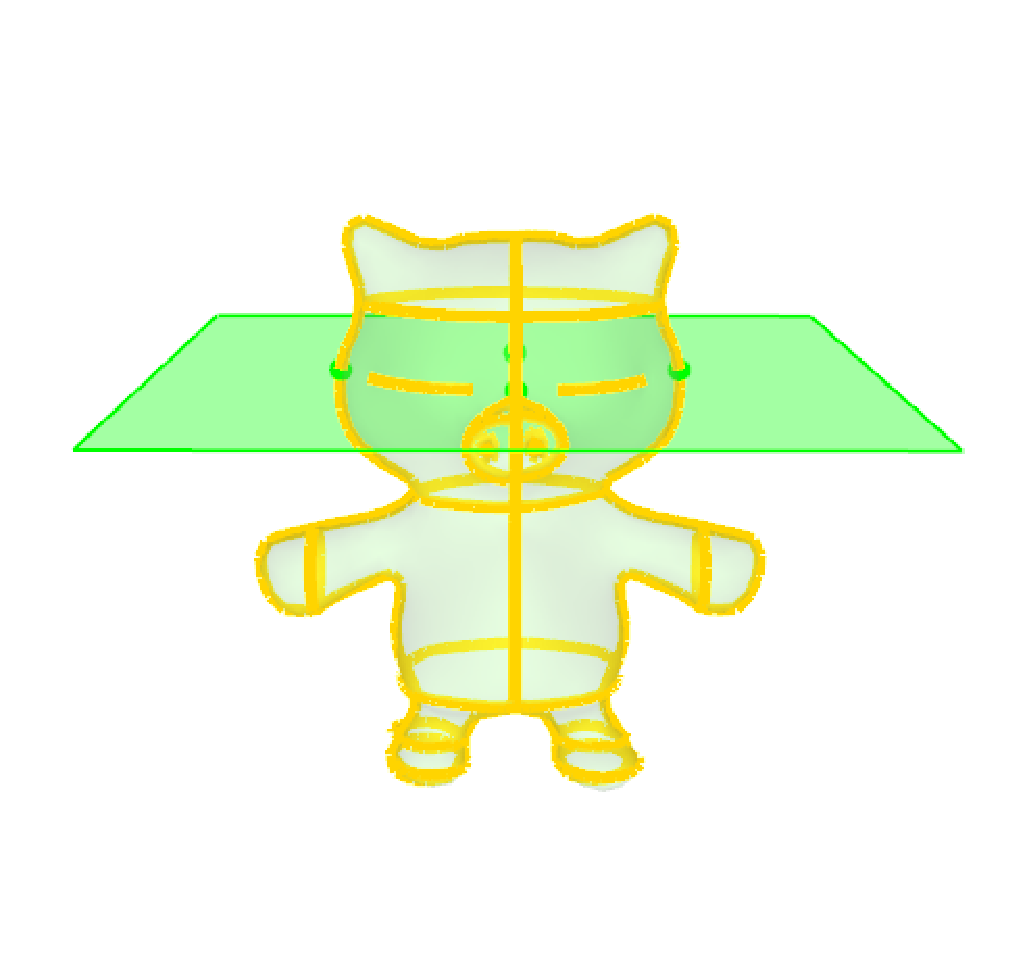
\includegraphics[scale=0.22]{figs/f3.pig-8.eps}
    \end{minipage}}
  \subfigure[]{
    \label{fig:pig:i}
    \begin{minipage}[b]{0.26\textwidth}
      \centering
      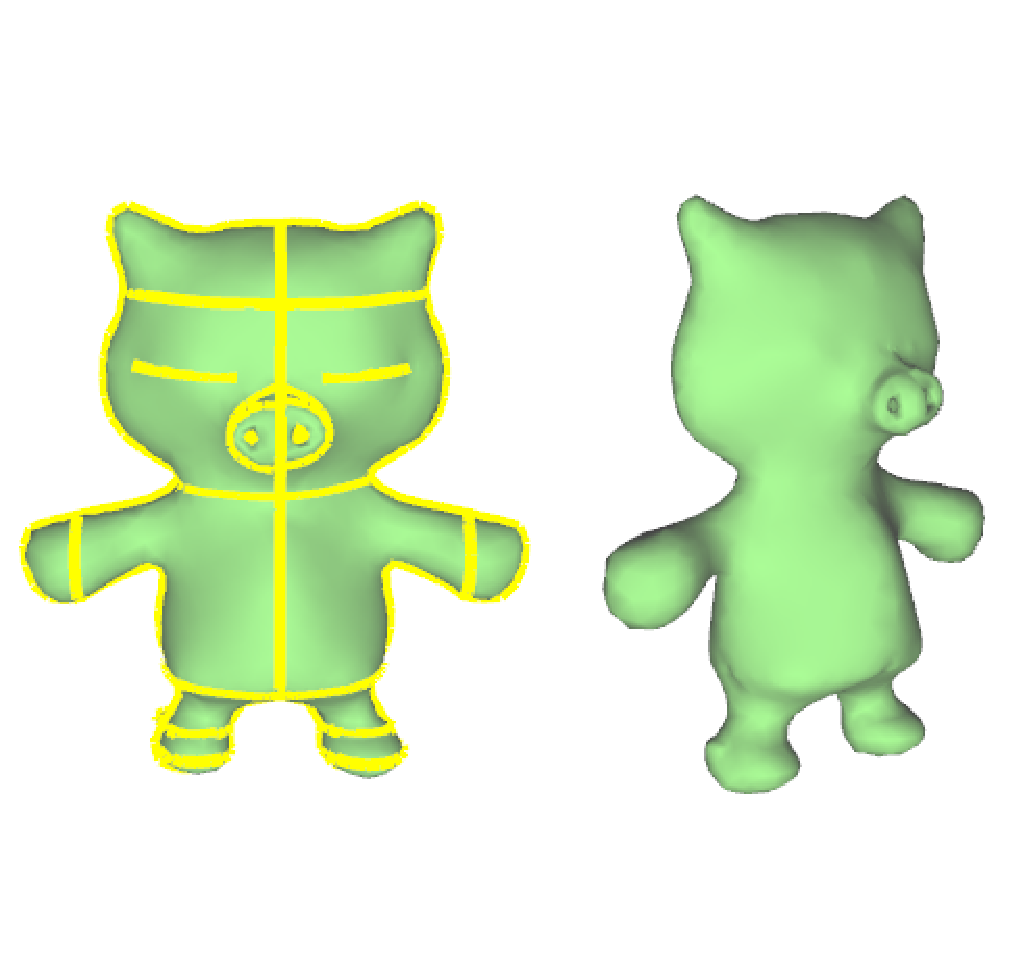
\includegraphics[scale=0.22]{figs/f3.pig-9.eps}
    \end{minipage}}
  \caption{Sketching tool. (a) Initially, three basic planes are provided; (b) A closed curve is sketched on the blue plane; (c) The preview of the reconstructed shape; (d) A new cross section is added on the red plane and the previewed shape is rendered; (e) The green plane is translated and three more cross sections are sketched; (f) More cross sections are added to refine the model; (g) The calculated cross section on the green plane is rendered semi-transparently to provide the user reference for further sketches; (h) Two incomplete cross sections are sketched on the green plane and the shape of the model is refined; (i) Final model.}
  \label{fig:pig} %% label for entire figure
\end{figure*}

%input of the system: cross sections on reference planes, why cross section
Our sketching tool provides the user three sets of orthogonal planes
as reference  planes. These reference planes are sketch planes, on
which the user can sketch the cross sections of the model. The word
\textit{cross section} means the intersection curve of the model
surface with a plane. We choose the cross section as the input of
the sketching tool for two considerations. First, it is an intuitive
and accurate description of a 3D model since it just lies on the
surface of the model. Comparing to other kinds of shape descriptors,
such as the silhouettes, it will cause less perception ambiguities
when the shape becomes complex. Second, a cross section is a planar
curve which can be quickly sketched in 3D space with the help of the
reference planes, and the sketching is thus simple yet effective for
depicting the 3D model. Meanwhile, taking the cross sections as the input
is also consistent with one of the visual rules in~\cite{HD00} that smooth
lines are usually interpreted as the contours of the 3D objects by human being.

%introduce reference planes
Initially, the $x=0$, $y=0$ and $z=0$ planes serve as the three
basic orthogonal planes. The user can define the cross sections of a
3D model by sketching strokes on any of these basic planes. These
three basic planes can also be translated along $x$, $y$ and $z$
axis respectively to allow the sketch of more contour curves. This
can result in several sets of parallel cross sections. Note that
though it is possible to rotate the basic planes to provide more
general reference planes and this could give the user more
flexibilities to sketch the contours, the price for this flexibility
is the algorithmic complexity of constructing 3D models from
non-parallel curve networks, the complexity of design and use of
interface, and the increase of occurrence of various ambiguities
from sketching. Therefore after a careful trade-off, we just allow
the basic planes to be translated and we find that this is generally
sufficient in practice for sketch-based freeform design.

%preview function, progresive modeling
The most distinguished feature of our system is the progressive
modeling function during sketching. That is, after the sketching on
one plane, the previewed up-to-date model which interpolates the
sketched strokes will be reconstructed and shown to the user. Since
comparing to the sculpting technique, sketching is an indirect way
of communicating with a shape, and it relies on the sense of human
perception~\cite{CIW08}, providing the previewed reconstruction
result can help the user to get a clear mind of the shape and
relative proportions of the constructed model after each sketch. It
also serves as a hint and reference on the following sketches and
makes the final shape conform to the user's expectation as much as
possible. Both the previewed model and the auxiliary planes are
rendered semi-transparently to avoid blocking the user's view on
existing sketches and the whole 3D space when providing sketching
references.

%auxiliary functions: operations on cross sections, highlighted intersection points, automatic view rotation
During the sketching process, all cross sections that  the user
sketched, as well as those calculated from the previewed model and
reference planes, are displayed and can be modified through
oversketching or deleted. Note that sketching cross sections on a
plane that intersects with the previewed shape looks similar to the
method adopted in~\cite{NSAC05,KSV09} at first glance, which shapes
a 3D model by iteratively oversketching its silhouette and deforming
it. However, the intrinsic difference lies in that the previewed
shape in our approach provides a reference for the following
sketches but sets little limitation on them, which means that these
sketches can be very flexible and the topology of the current shape
may even be changed. While in the deformation method the sketches
are restricted by the 3D model to be correspondence with the
existing cross sections on it, thus only the geometry of the current
shape can be modified.

%partial cross section
Since forcing the user to sketch complete cross sections may be
troublesome and inaccurate, we also allow the input to be just a
part of the cross section. Of course, such a stroke is to some
extent arbitrary and may not be explained as a valid part of the
cross section of the model to create. We thus set some requirements
for such an input and try to make it valid (see the details in
Section~\ref{ch4:sec:disc}).

%automatic view rotation
The system is also able to automatically rotate the view to make
the user selected plane for sketching face him as much as possible.
This is inspired by the observation in~\cite{BBS08} that a good view
for the user to sketch the 2D strokes is the one that has a large
visible projection. With this function, frequent manual viewpoint
changes which may interrupt the user's attention on the sketching
can be avoided.

%example
Figure~\ref{fig:pig} shows an overview of the creation process. With
 help of the reference planes and shapes, more descriptions on the
shape of a model can be sketched and perception ambiguities can be
reduced. This minimizes the unnecessary back and forth adjustment of
the sketches and speeds up the production process of a 3D model.

%cad system --> our system
It is noticed that our interface is similar to that in traditional
3D modeling software which provides the user three orthogonal views
to implement the modeling operations. This will make it easy to use
for users who are familiar with this type of interface. Moreover,
comparing to the system in~\cite{RDI10} which lets the user  sketch
the silhouettes of a 3D model on three orthogonal views, we give the
user the freedom to input more shape descriptions in 3D space, such
that less imagination will be needed when creating a 3D model with
multiple components and different depths.

%ambiguity and stroke rules
It should be pointed out that even though references have been
provided for defining the shape of a model, sometimes ambiguity
still occurs. The ambiguity arises from two aspects: the user input
strokes may not necessarily follow the same style -- different users
may have different manners for defining the shape of a model; even
with the same contours, the understandings of the shape they defined
may vary among different users. So some rules must be provided for
sketching the cross sections. The details of the rules will be
discussed in Section~\ref{ch3:sec:algo:rule}.

%-------------------------------------------------------------------------
\subsection{Sculpting tool}
\label{ch3:sec:ui:sculpt}

%sculpting functions
After the user sketches the general shape of the  model, we provide
a series of sculpting functions for him/her to do further
refinement. The sculpting tools include deformation, extrusion,
tunneling (digging a hole), cutting and smoothing functions, all of
which are based on the user's sketches. An intelligent stroke
recognition mechanism is used to judge the user's intention
according to the sketches and switch to the corresponding mode
automatically.

\subsubsection{Basic functions}
\label{Sec:UI:sculpt:mode}

\begin{figure} [htbp]
  \centering
  \subfigure[]{
    \centering
    \label{fig:sculpt:create} %% label for first subfigure
    \begin{minipage}[b]{0.45\textwidth}%0.45
      \centering
      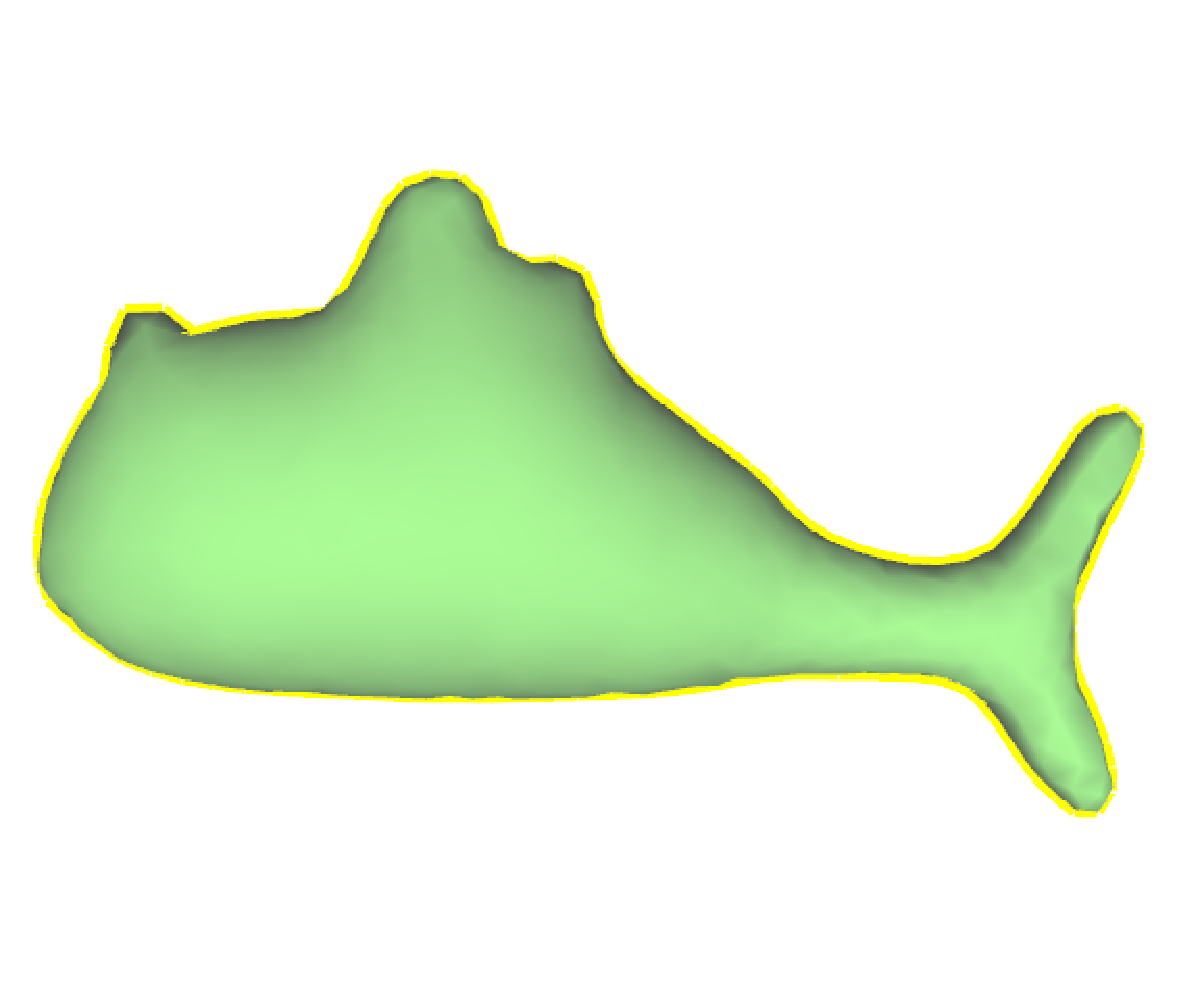
\includegraphics[scale=0.11]{figs/f3.fish-sculpt-1.eps}%0.12
    \end{minipage}}
   \subfigure[]{
    \centering
    \label{fig:sculpt:tunnel} %% label for first subfigure
    \begin{minipage}[b]{0.51\textwidth}%0.45
      \centering
      \includegraphics[scale=0.11]{figs/f3.fish-sculpt-2.eps}%0.1
    \end{minipage}}
   \subfigure[]{
    \centering
    \label{fig:sculpt:extrude} %% label for first subfigure
    \begin{minipage}[b]{0.48\textwidth}%0.38
      \centering
      \includegraphics[scale=0.11]{figs/f3.fish-sculpt-3.eps}%0.11
    \end{minipage}}
   \subfigure[]{
    \centering
    \label{fig:sculpt:cut} %% label for first subfigure
    \begin{minipage}[b]{0.48\textwidth}%0.5
      \centering
      \includegraphics[scale=0.11]{figs/f3.fish-sculpt-4.eps}%0.11
    \end{minipage}}
   \subfigure[]{
    \centering
    \label{fig:sculpt:smooth} %% label for first subfigure
    \begin{minipage}[b]{0.9\textwidth}%0.38
      \centering
      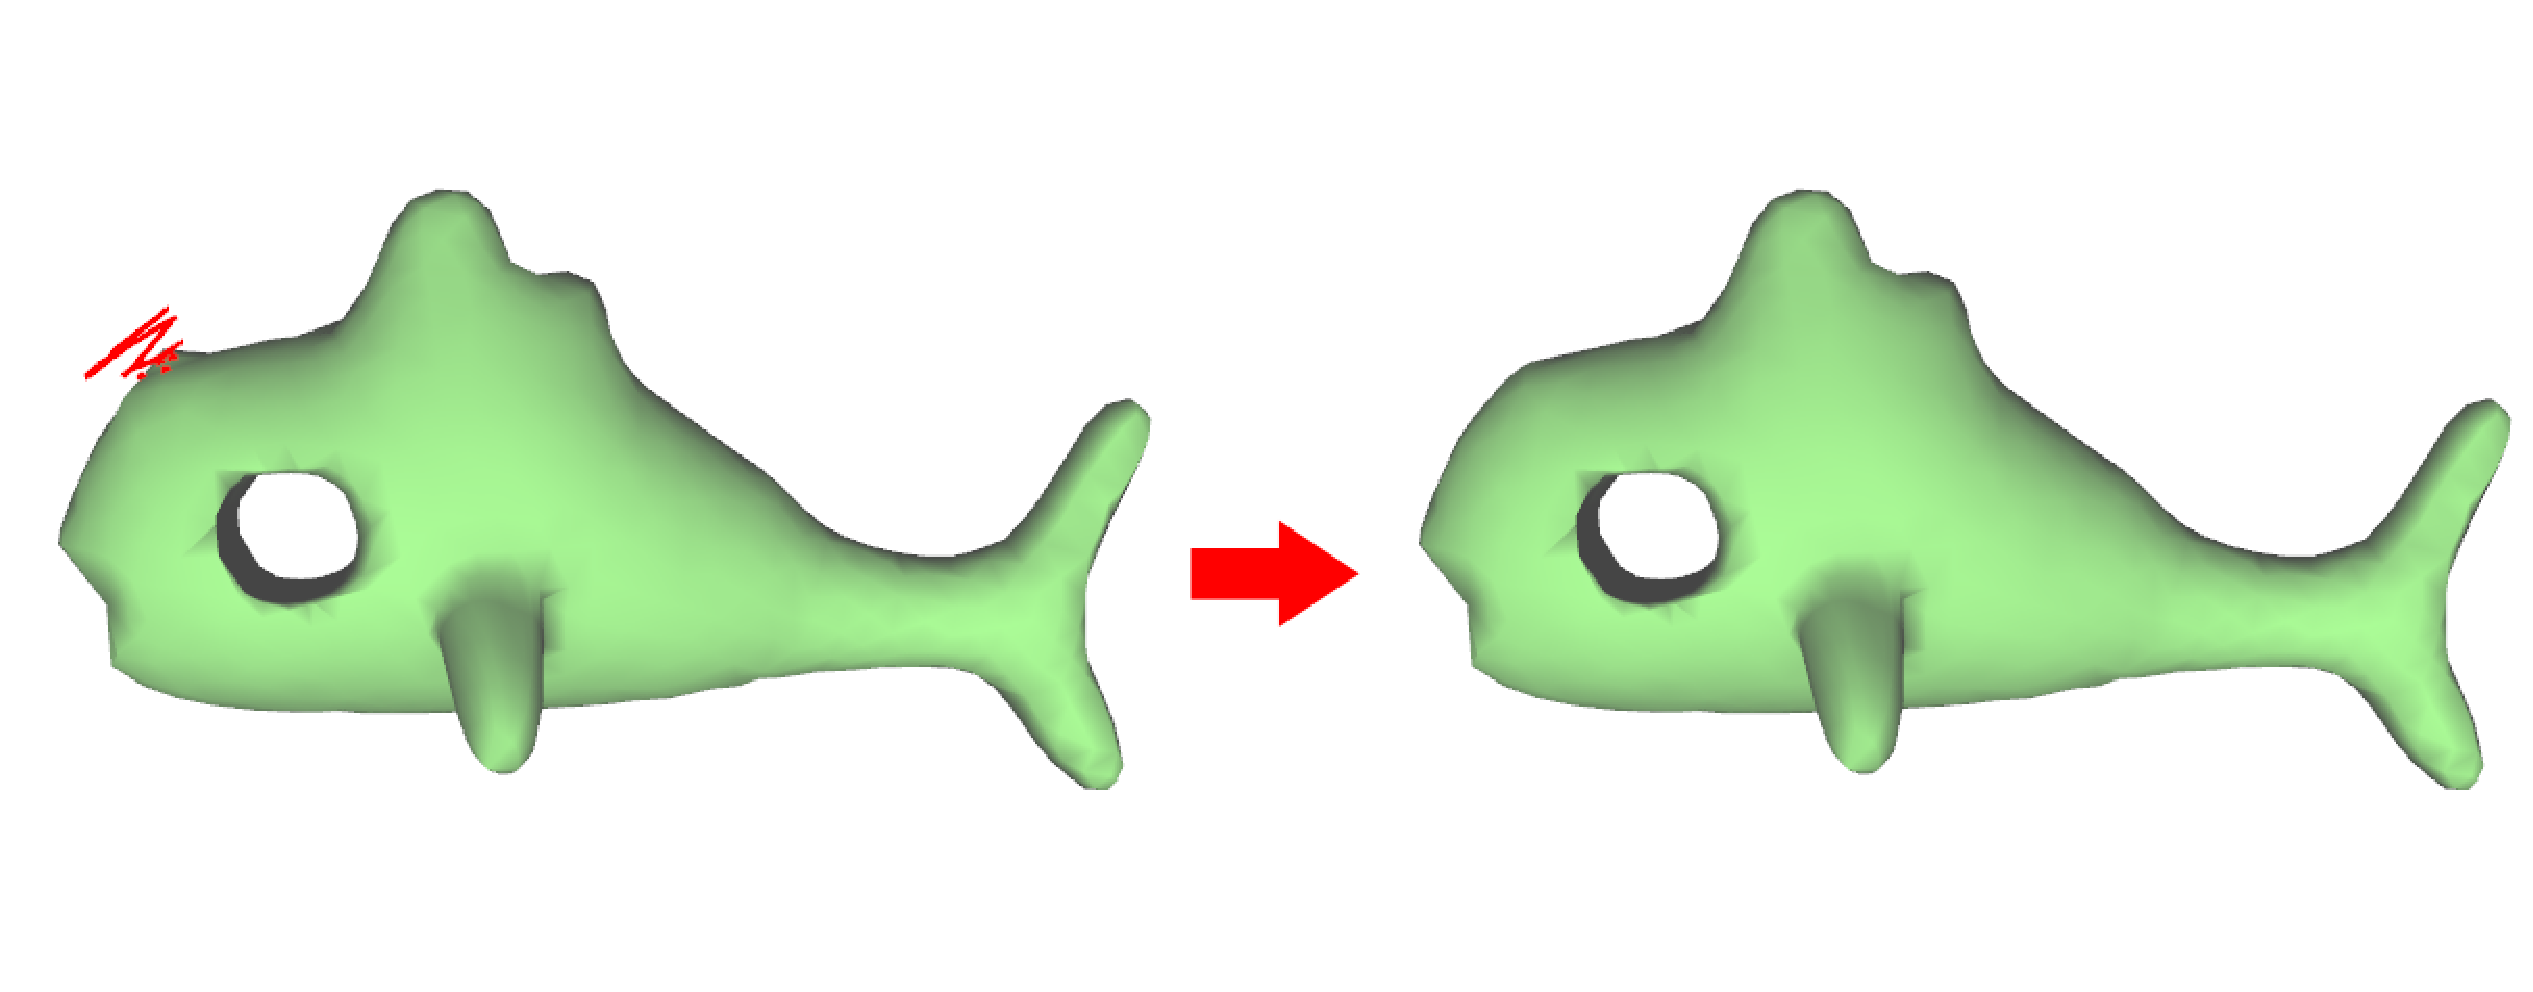
\includegraphics[scale=0.11]{figs/f3.fish-sculpt-5.eps}%0.11
    \end{minipage}}
  \caption{Sculpting tools. (a) The user sketched cross section (yellow) and initially generated model; (b) Tunneling operation; (c) Extrusion operation; (d) Cutting operation; (e) Smoothing operation.}
  \label{fig:sculpt} %% label for entire figure
\end{figure}

%stroke types. open stroke
The stroke set our system accepts in the sculpting tool includes
three general types: a simple open stroke, a closed stroke, and a
scratch-out stroke. When a simple open stroke is sketched, the
operation may be cutting or deformation, depending on whether the
stroke passes across the model in the image space or not. If it is a
cutting stroke, a following stroke will be required to indicate
which part to cut off (Figure~\ref{fig:sculpt:cut}). The subsequent
operation of deformation will be introduced in detail in
Section~\ref{ch3:sec:ui:sculpt:deform}.

%closed strokes, extrusion or tunneling
We allow the user to extrude or dig  a part similar to the operation
in~\cite{IMT99,NISA07} when a closed stroke is sketched on the
surface of the model. What is different, our system automatically
generates a reference plane orthogonal to the closed curve, on which
the user can draw the silhouette curve of the extruded/dug part
(Figure~\ref{fig:sculpt:extrude}). This plane can be rotated about
two axes: the line passing through the center of the closed stroke
and orthogonal to the stroke as much as possible or the line
connecting the first drawn point of the closed stroke and the
farthest point to it on the stroke. The reference plane helps to
confirm the position of the silhouette curve and gives flexibility
to adjust its direction. When the silhouette curve intersects with
the backside surface, the operation turns to tunneling and a hole is
dug (Figure~\ref{fig:sculpt:tunnel}).

%scratch strokes, smoothing
When the user scratches a part on the model back and  forth, it is
regarded as a smoothing operation and the local part will be
smoothed (Figure~\ref{fig:sculpt:smooth}).


\subsubsection{Deformation tool}
\label{ch3:sec:ui:sculpt:deform}

\begin{figure*} [htbp]
  \centering
  \subfigure[]{
    \centering
    \label{fig:deform:a} %% label for first subfigure
    \begin{minipage}[b]{0.3\textwidth}
      \centering
      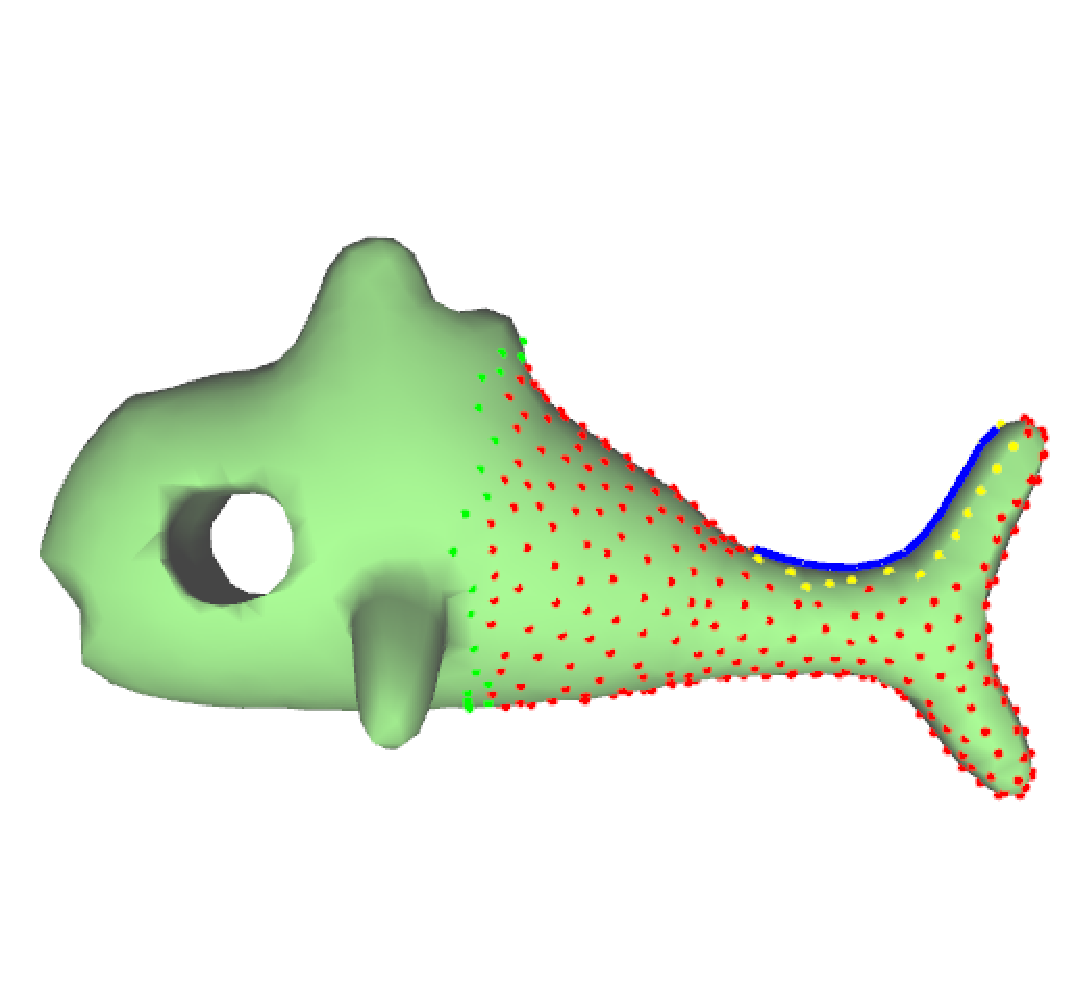
\includegraphics[scale=0.15]{figs/f3.fish-deform-1.eps}
    \end{minipage}}
  \subfigure[]{
    \centering
    \label{fig:deform:b}
    \begin{minipage}[b]{0.3\textwidth}
      \centering
      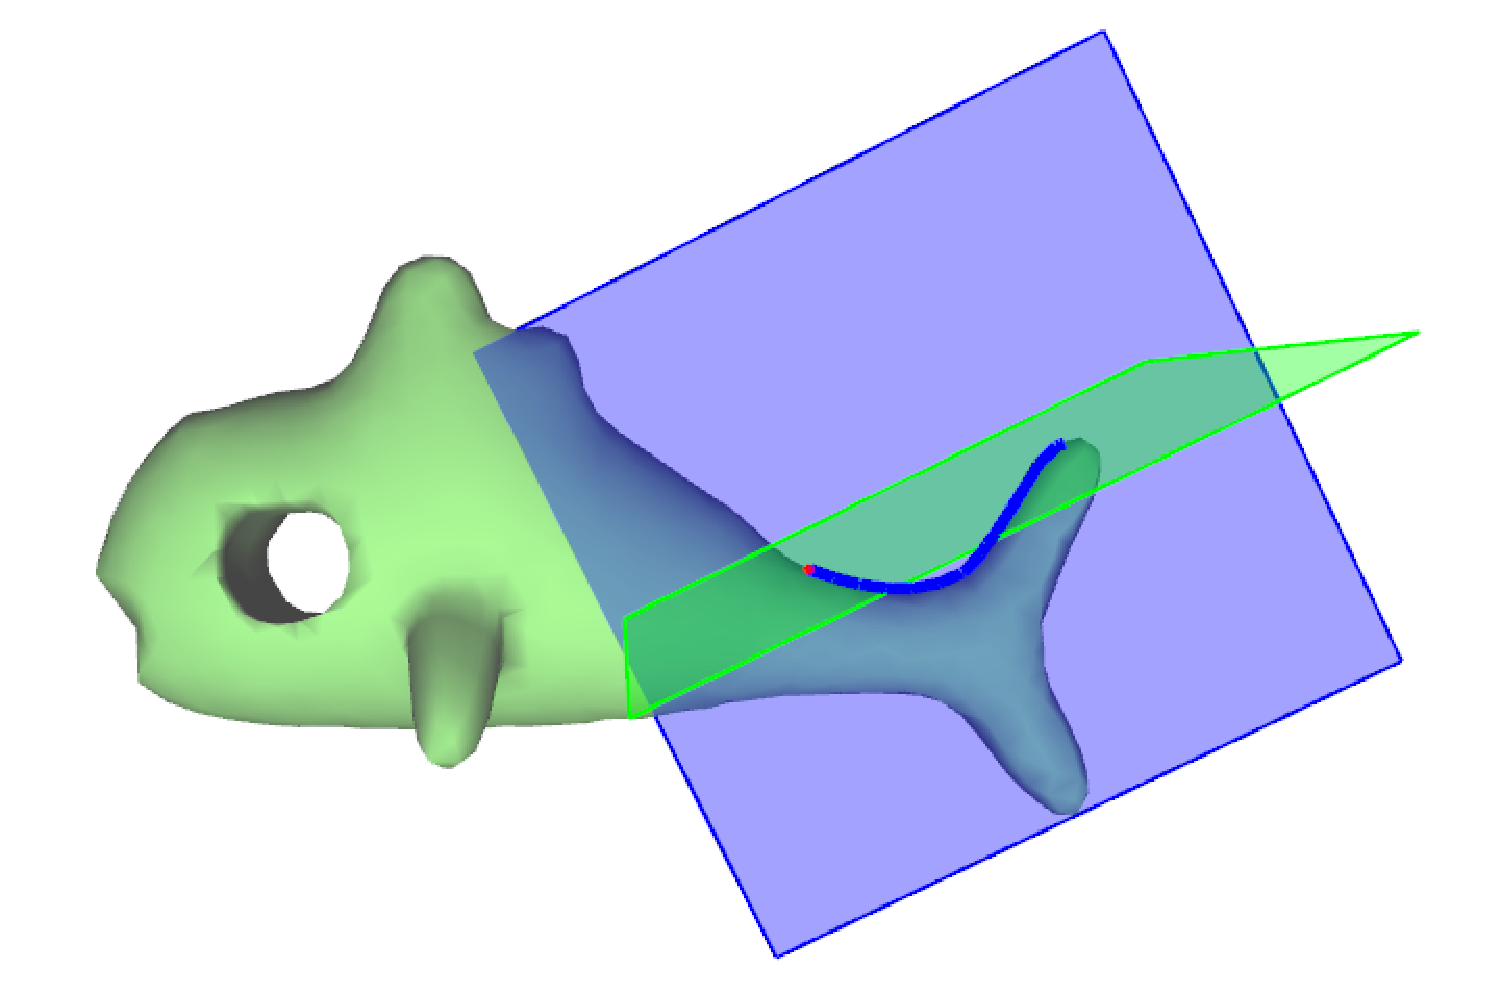
\includegraphics[scale=0.15]{figs/f3.fish-deform-2.eps}
    \end{minipage}}
  \subfigure[]{
    \centering
    \label{fig:deform:c}
    \begin{minipage}[b]{0.3\textwidth}
      \centering
      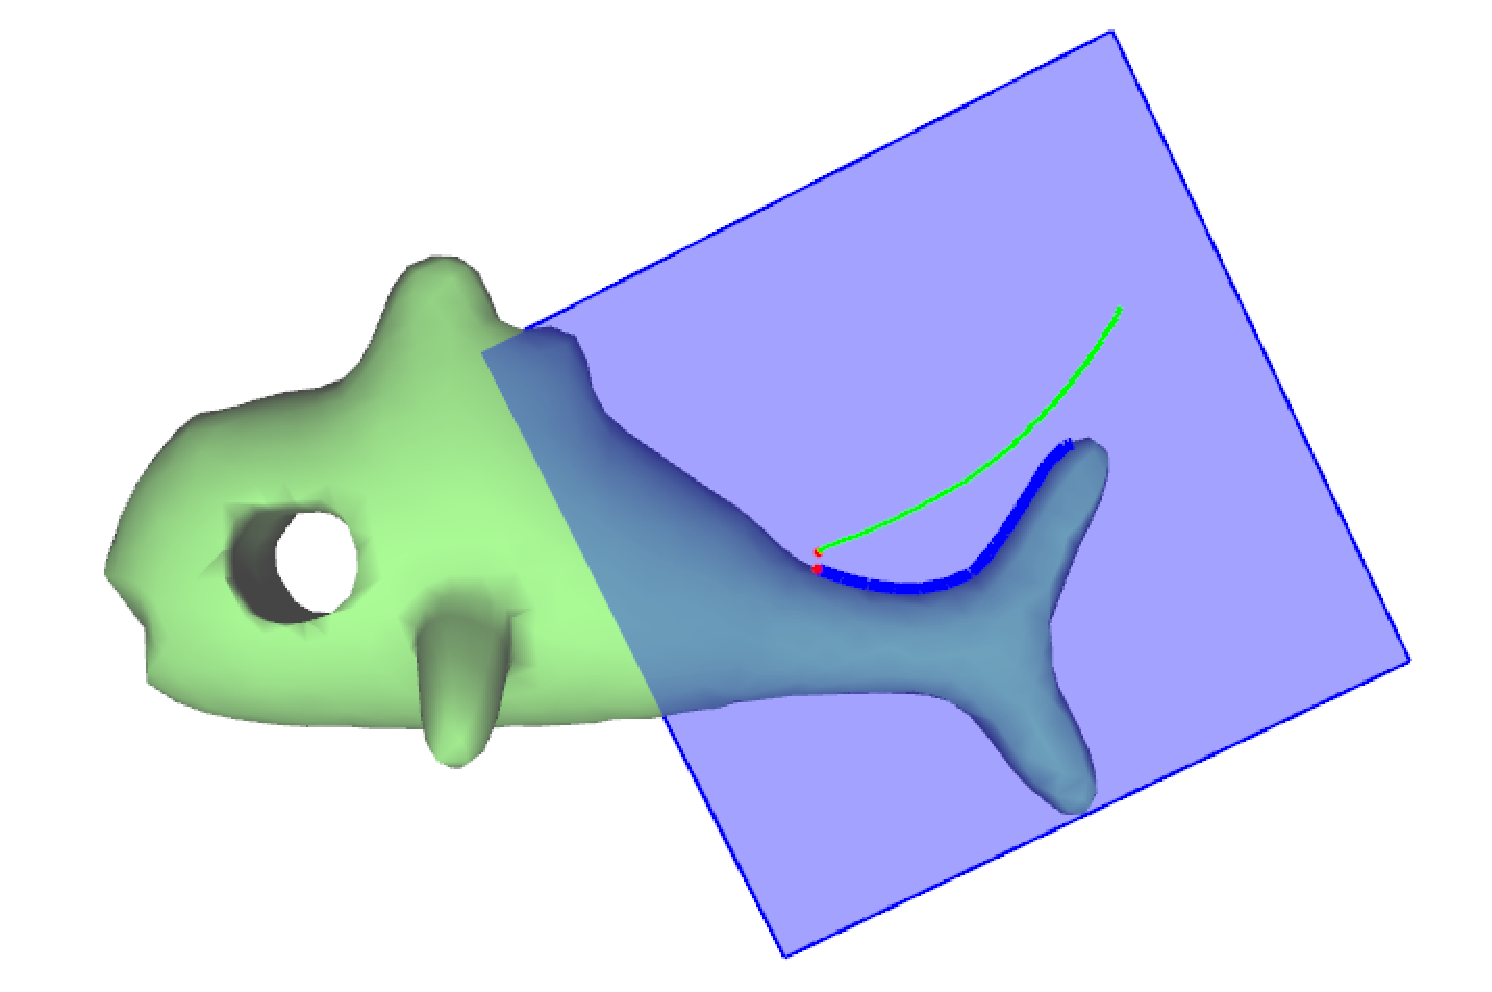
\includegraphics[scale=0.15]{figs/f3.fish-deform-3.eps}
    \end{minipage}}
  \subfigure[]{
    \label{fig:deform:d}
    \begin{minipage}[b]{0.3\textwidth}
      \centering
      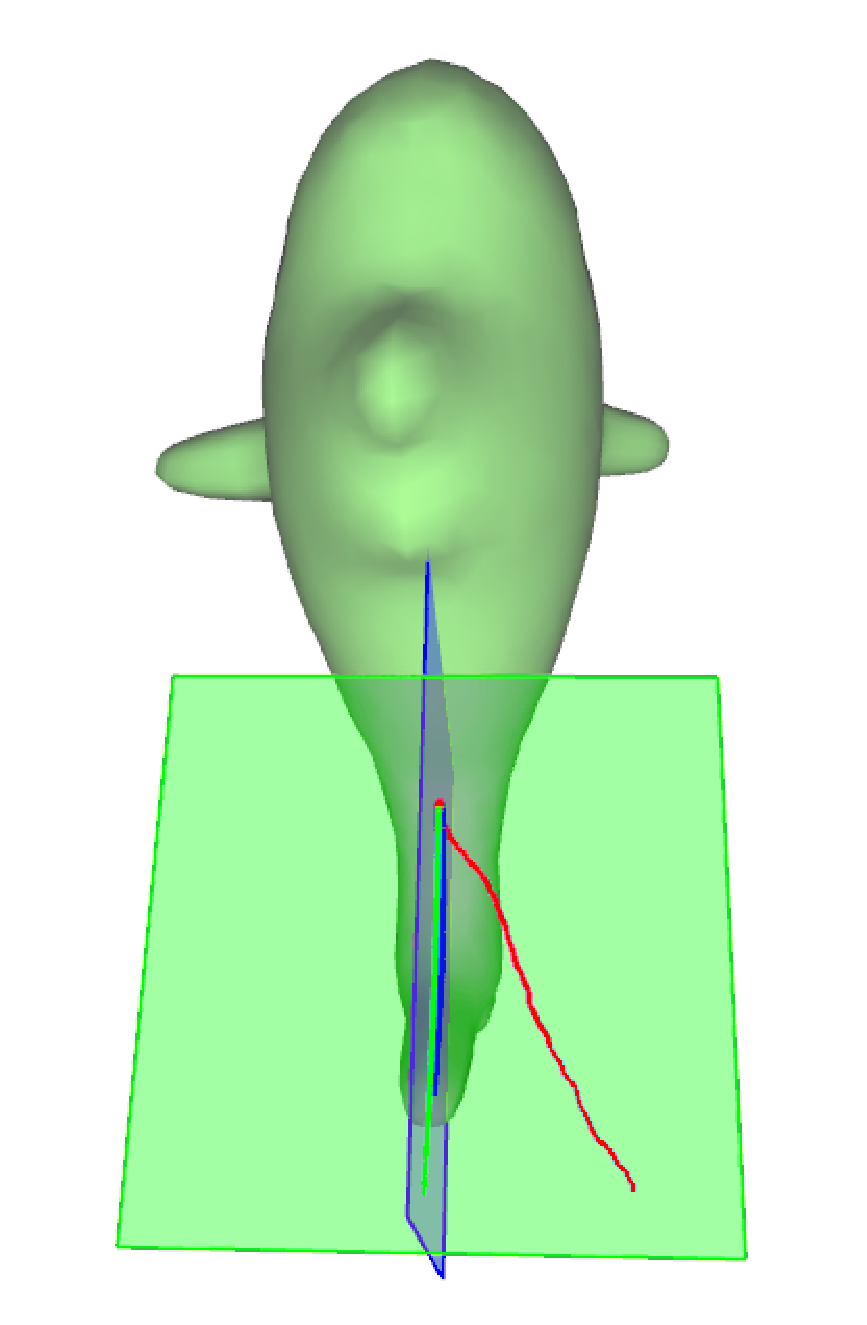
\includegraphics[scale=0.15]{figs/f3.fish-deform-4.eps}
    \end{minipage}}
  \subfigure[]{
    \label{fig:deform:e}
    \begin{minipage}[b]{0.3\textwidth}
      \centering
      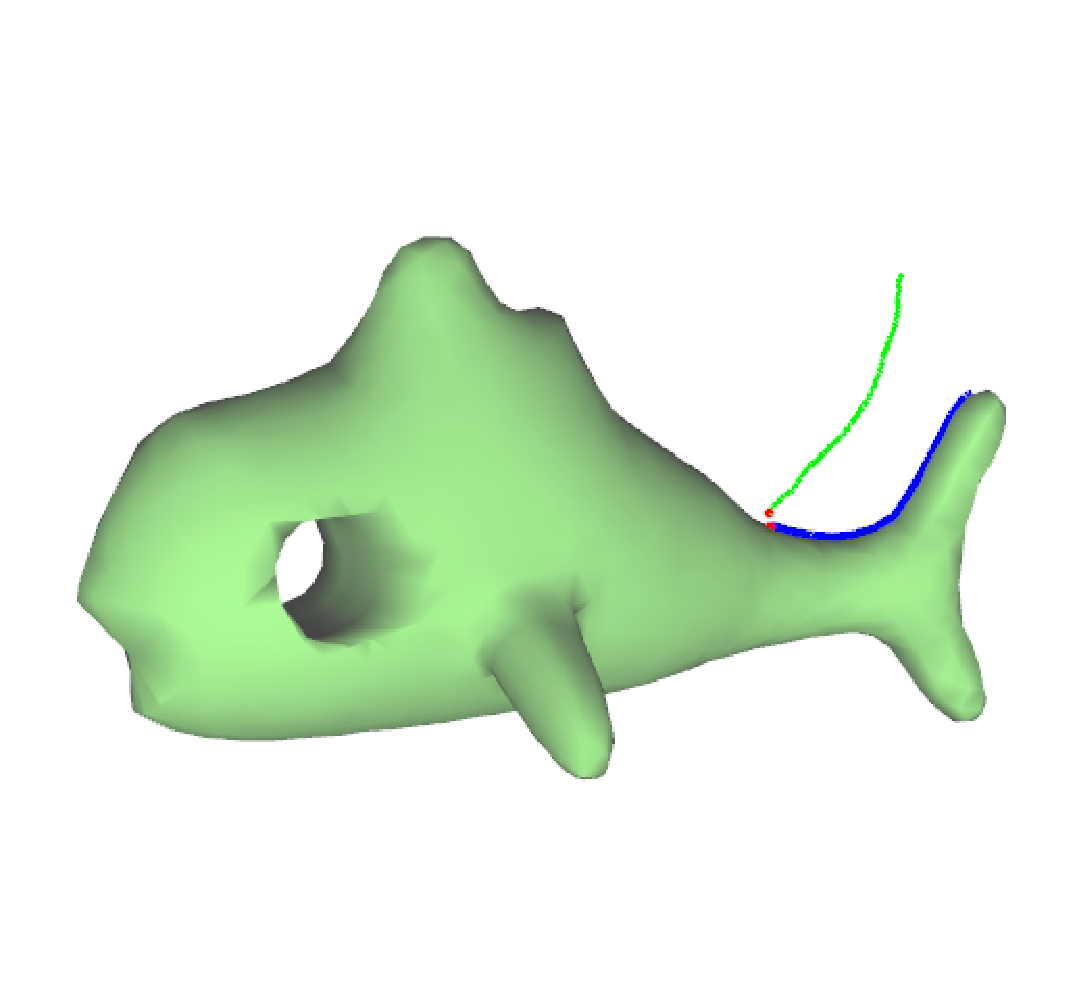
\includegraphics[scale=0.15]{figs/f3.fish-deform-5.eps}
    \end{minipage}}
  \subfigure[]{
    \label{fig:deform:f}
    \begin{minipage}[b]{0.3\textwidth}
      \centering
      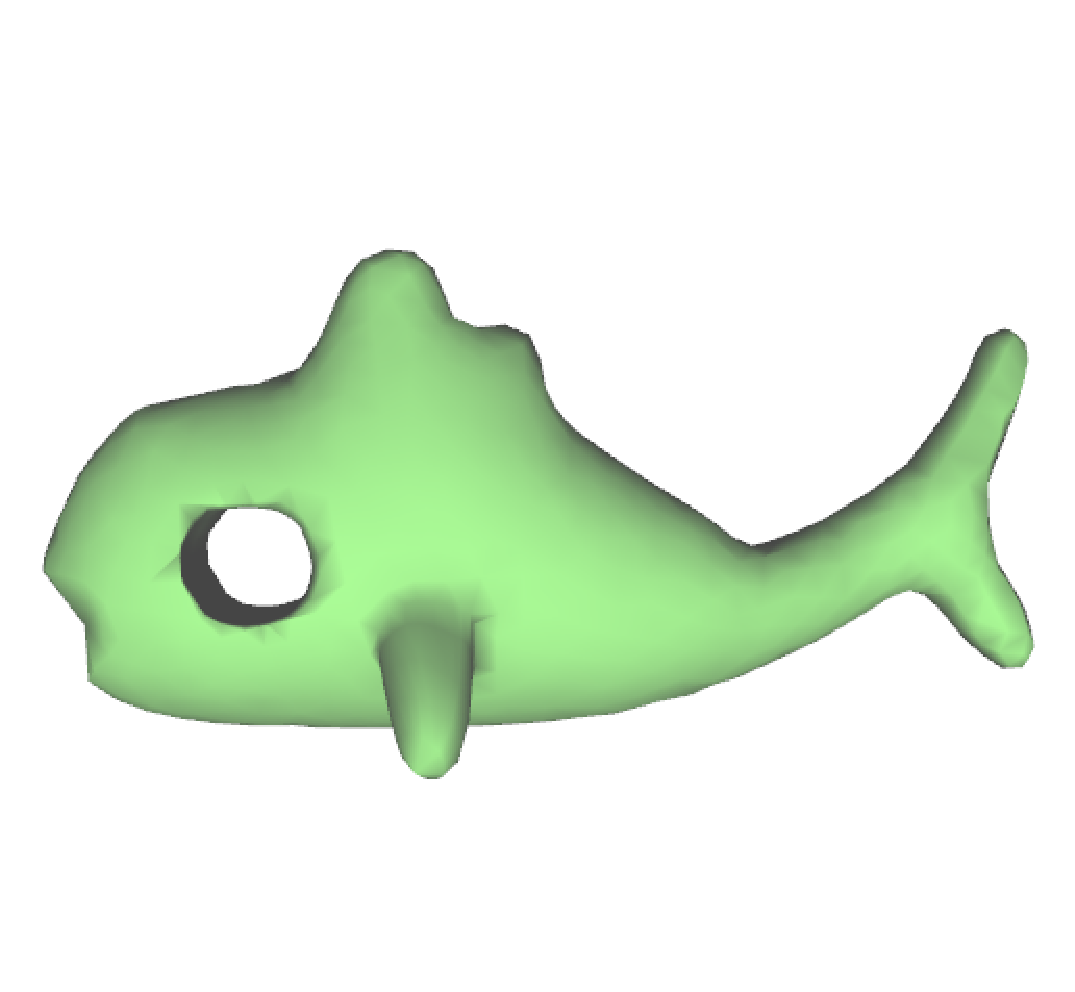
\includegraphics[scale=0.15]{figs/f3.fish-deform-6.eps}
    \end{minipage}}
  \caption{An example of using the deformation tool. (a) The blue curve is the handle curve sketched on the initial model. The yellow, red and green dots denote the handle, ROI and static vertices respectively; (b) The automatically generated base plane (blue) and projection plane (green); (c) The new curve (green) drawn on the base plane; (d) A curve (red) is drawn on the projection plane to create a non-planar new curve; (e) The updated new curve (green); (f) The deformed model.}
  \label{fig:deform} %% label for entire figure
\end{figure*}

%introduction of deformation, why handle curve instead of point
The deformation tool is an important  sculpting function in our
system. As introduced in Section~\ref{ch2:sec:sbim:sculpt}, to
deform a mesh, a handle needs to be first specified for the
following operations. Here we use a curve as the handle instead of a
point, since it contains multiple points and thus provides more
flexibility for the manipulation. The user needs to first sketch a
stroke which will be projected onto the mesh to generate the handle
curve. Two reference planes will then be generated automatically.
Next, the user needs to sketch on the reference planes to specify
the new shape and position of the handle curve, after which the
deformation is completed. To implement this deformation process, the
following information should be specified: a set of vertices (called
handle vertices) and their new positions; the vertices within a
region of interest (ROI), which will move with the handles; and the
vertices will remain unchanged during the deformation process
(called the static vertices).

%how to compute handle curve
To generate the handle curve, we use a method similar to that
in~\cite{NSAC05}. The handle curve is composed of handle vertices.
The vertices of the edges or faces on which the projection of the
input stroke lie are regarded as the handle vertices. See
Figure~\ref{fig:deform:a} for an illustration.

%new position of handle curve
The specification of new positions of the handle  vertices seems not
trivial. Unlike previous existing methods, we provide the user with
two reference planes for the sketching of the new curve: a base
plane which passes the handle vertices as many as possible for
sketching the basic shape of the new curve and a projection plane,
which is orthogonal to the base plane, for drawing the projection of
the new curve (Figure~\ref{fig:deform:b}). In general, the base
plane is sufficient for sketching the new shape of the handle curve.
However, if the new handle curve is desired to be non-planar, the
projection plane is used to sketch its projection and then the new
handle curve is determined (Figure~\ref{fig:deform:c} -
Figure~\ref{fig:deform:e}). In addition, in our system the two
planes can also be rotated to provide more flexibility. In this way,
the user can draw arbitrary curves in 3D space while being fully
aware of the locations.

%ROI vertices
For selection of the ROI vertices, three methods  are available. A
simple approach is to specify a threshold and vertices whose
Euclidean distances to the handles below this threshold are regarded
as the ROI vertices. Another approach is to let user draw a circle
on the 2D screen. The ROI vertices are the ones whose projections
onto the screen are inside the circle. However these two methods
seem not quite precise when the selection of certain vertices is
required for relatively complex models. So we provide a new tool --
a brush, to make the selection process somewhat like brushing on a
model. The vertices brushed will then be chosen as the ROI vertices.
The brush can be viewed as a complementary tool for the former two
methods. The user could take a rough selection using the first two
tools and then make further modifications by brushing on the model.

These sculpting tools are all sketch-based and quite convenient to
use. Together with the sketching tool, a complete modeling system is
built up. With this system, the user could easily create and edit a
3D object in a short period by sketching strokes.


%-------------------------------------------------------------------------
\section{Algorithms}
\label{ch3:sec:algo}

In this section we describe the underlying algorithms of the
sketching interface. We first introduce the preprocessing algorithm
for the input strokes. Then we propose the stroke rules for
interpreting input cross sections and making them valid for the
computation of the 3D model. Finally the  algorithm for the
calculation of the reference planes in the sculpting tool is
provided.

%-----------------------------------------------------------------------------------------------------------------
\subsection{Input stroke preprocessing}\label{ch3:sec:alg:strokepreproc}

For sketch-based modeling systems, the original input stroke created
from an input device usually cannot be used directly due to two
reasons: 1). The points of the stroke are noisy because of the shaky
nature of handling the input devices; 2). the spatial and temporal
quantization of the input by the hardware may contain error since
the speed that the user draws is random. Thus, we perform a
three-step preprocessing of the input stroke in each functions, as
shown in Figure~\ref{fig:alstrokeproc}.

\begin{figure} [htbp]
  \centering
  \subfigure[]{
    \centering
    \label{fig:alstrokeproc:a} %% label for first subfigure
    \begin{minipage}[b]{0.2\textwidth}
      \centering
      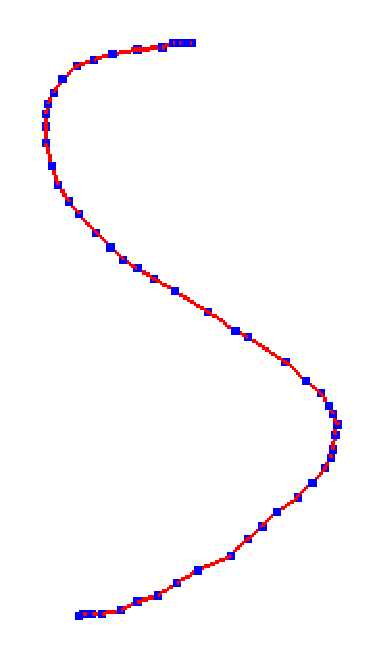
\includegraphics[scale=0.3]{figs/f3.strokepre-1.eps}
    \end{minipage}}
  \subfigure[]{
    \centering
    \label{fig:alstrokeproc:b}
    \begin{minipage}[b]{0.2\textwidth}
      \centering
      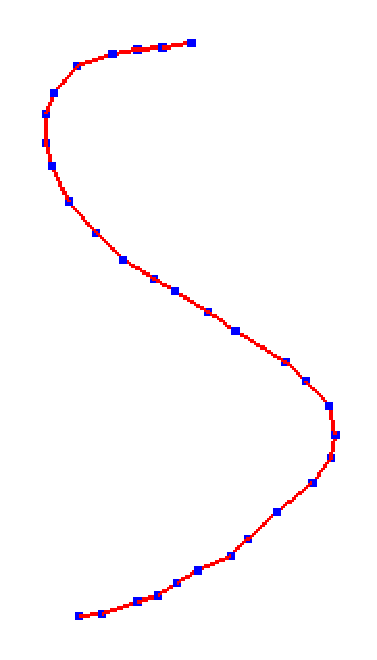
\includegraphics[scale=0.3]{figs/f3.strokepre-2.eps}
    \end{minipage}}
  \subfigure[]{
    \centering
    \label{fig:alstrokeproc:c}
    \begin{minipage}[b]{0.2\textwidth}
      \centering
      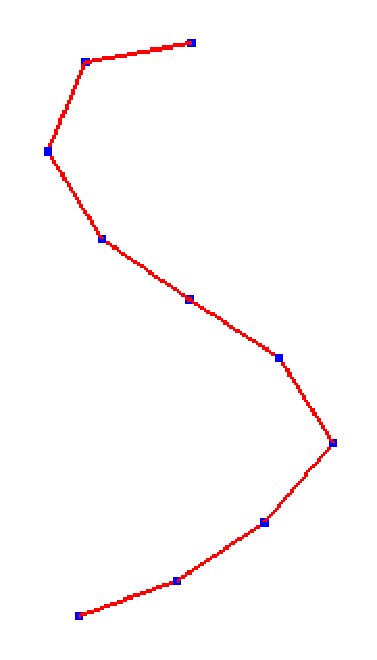
\includegraphics[scale=0.3]{figs/f3.strokepre-3.eps}
    \end{minipage}}
  \subfigure[]{
    \centering
    \label{fig:alstrokeproc:d}
    \begin{minipage}[b]{0.2\textwidth}
      \centering
      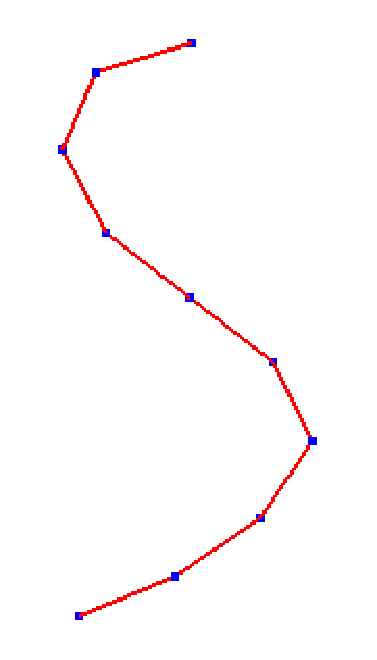
\includegraphics[scale=0.3]{figs/f3.strokepre-4.eps}
    \end{minipage}}
  \caption{Stroke Preprocessing: The goal here is to filter the noisy points and get a smooth curve with 10 points. (a) Initial input; (b) Filtering result; (c) Resampling result; (d) Final result after smoothing.}
  \label{fig:alstrokeproc} %% label for entire figure
\end{figure}

First of all, a point whose distance to its previous one is less
than a given threshold will be judged as a redundant noisy point and
deleted.

Then we resample the stroke to make its points number a  predefined
value $N_{pre}$. To do this, we first calculate the summed distance
$S_{total}$ between each two points to get the length of the stroke.
Then through dividing $S_{total}$ by $N_{pre}$, we get the expected
unit distance $S_{unit}=S_{total} / N_{pre}$ along the route of the
stroke between each two new points. Finally starting from the first
point, we \lq\lq{travel}\rq\rq along the original stroke trajectory.
Every time when a unit distance $S_{unit}$ reaches, we position a
new stroke point. The \lq\lq{journey}\rq\rq ends until the last new
point is placed. A new curve is then formed.

This simple resampling algorithm can produce a stroke with a desired
number of points. The original shape of the stroke is preserved as
much as possible. Meanwhile, it is quite easy to implement and
avoids complicated computations required in some existing methods
(for example, fitting a polyline to a B-spline and evenly sample
it~\cite{CMZHB99}).

Finally the stroke is smoothed by moving each point according to Eq.~\ref{eq:strokesmooth}.

\begin{equation}
\label{eq:strokesmooth}
    P_i^\prime = \frac{P_{i-1}+4*P_i+P_{i+1}}{6}
\end{equation}
where $P_i$ and $P_i^\prime$ are the old and new positions of point
$i$. $P_{i-1}$ and $P_{i+1}$ are the old positions of its two
neighbor points.

The stroke preprocessing is a fundamental step for the functions in
the system and helps to produce a visually-pleasant 3D model.


\subsection{Stroke rules}
\label{ch3:sec:algo:rule}

As mentioned in Section~\ref{Sec:UI:sketch}, to avoid the
perception ambiguity, some rules are needed to regularize and
interpret the user sketched strokes before we construct the surface.
It is suggested in the guidelines for the user interface design
in~\cite{MN90} that the interface should match with the real world
conventions, which is coincident with the user psychology that the
user always prefer familiar concepts rather than system-oriented
terms~\cite{GC87,DA06}. Thus, these stroke rules should make the
input curves consistent with the common sense of the cross sections
which represent the intersections of the planes and the surface
of a 3D object with no self-intersections. Specifically, these
rules include:

\begin{enumerate}
    \item For curves on a plane, if they do not intersect with or contain each other, the interior of each curve belongs to the interior of the model.
    \label{rule:1}
    \item For two curves $S_1$ and $S_2$ on a plane, if $S_1$ is totally contained in $S_2$, then it means that the intersection between the plane and the model is a ring. If the containing relationship exists among more than two curves, that is, we have $n$ curves $S_1,S_2,...,S_n$ and $S_i$ is within $S_{i+1}$, then we start the perception from the outermost pair of curves $S_n$ and $S_{n-1}$.
    \label{rule:2}
    \item If a curve is self-intersected or intersects with any other curves lying on the same plane, then it is treated as an invalid curve and thus discarded.
    \label{rule:3}
    \item For two curves $S_1$ and $S_2$ lying on two orthogonal planes $P_1$ and $P_2$ respectively, the intersection point set $\{V_{S_1P_2}\}$ of curve $S_1$ and plane $P_2$, must be exactly the \emph{same} as the set $\{V_{S_2P_1}\}$ of $S_2$ and plane $P_1$.
    \label{rule:4}
\end{enumerate}

Next we give some explanations of these rules.  The first rule is
easy to understand. When a user draws one or more closed strokes,
the strokes are usually regarded as the outer contours of an object.

When a user tries to make a hole on the mesh surface  to create a
relatively complex model, a pair of curves are often used, of which
one is contained in the other. The ring between the two curves is
the interior part of the model. If more holes are desired, more
pairs of curves should be used. To avoid the ambiguity of
perception, the order of analysis is inward starting from the
outermost pair. For example, suppose we have $n$ curves
$S_1,S_2,...,S_n$ and $S_{i-1}$ is totally contained in  $S_i$. Then
$S_n$ and $S_{n-1}$ form a ring, $S_{n-2}$ and $S_{n-3}$ form
another ring which is contained in the previous one, and so on. If
$n$ is an even number, then the ring formed by $S_2$ and $S_1$ is
innermost; Otherwise we just apply rule~\ref{rule:1} to $S_1$ -- the
interior of $S_1$ is the interior of the model. An example of
rule~\ref{rule:2} is shown in Figure~\ref{fig:rule2}.
Rule~\ref{rule:2} makes it possible to model a mesh with arbitrary
topology directly by sketching the contours at the creation phase.

\begin{figure} [htbp]
  \centering
  \subfigure[]{
    \centering
    \label{fig:rule2:a} %% label for first subfigure
    \begin{minipage}[b]{0.22\textwidth}
      \centering
      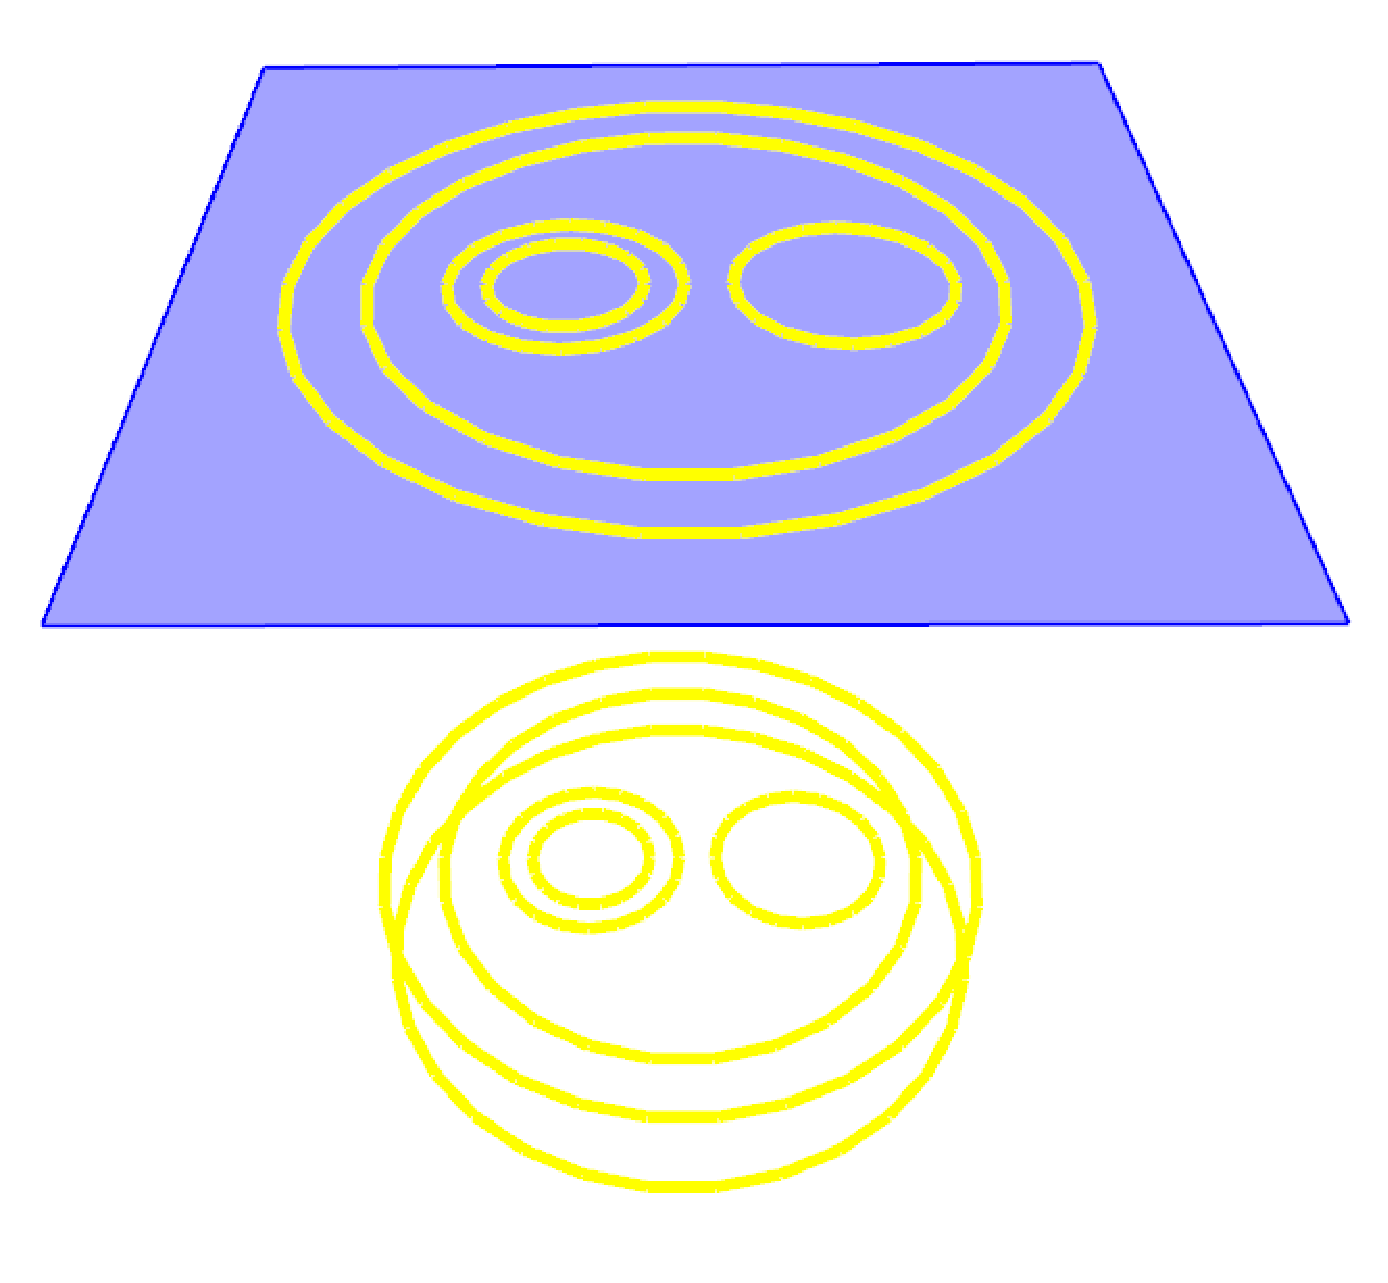
\includegraphics[scale=0.12]{figs/f3.rule2-1.eps}
    \end{minipage}}
  \subfigure[]{
    \centering
    \label{fig:rule2:b}
    \begin{minipage}[b]{0.22\textwidth}
      \centering
      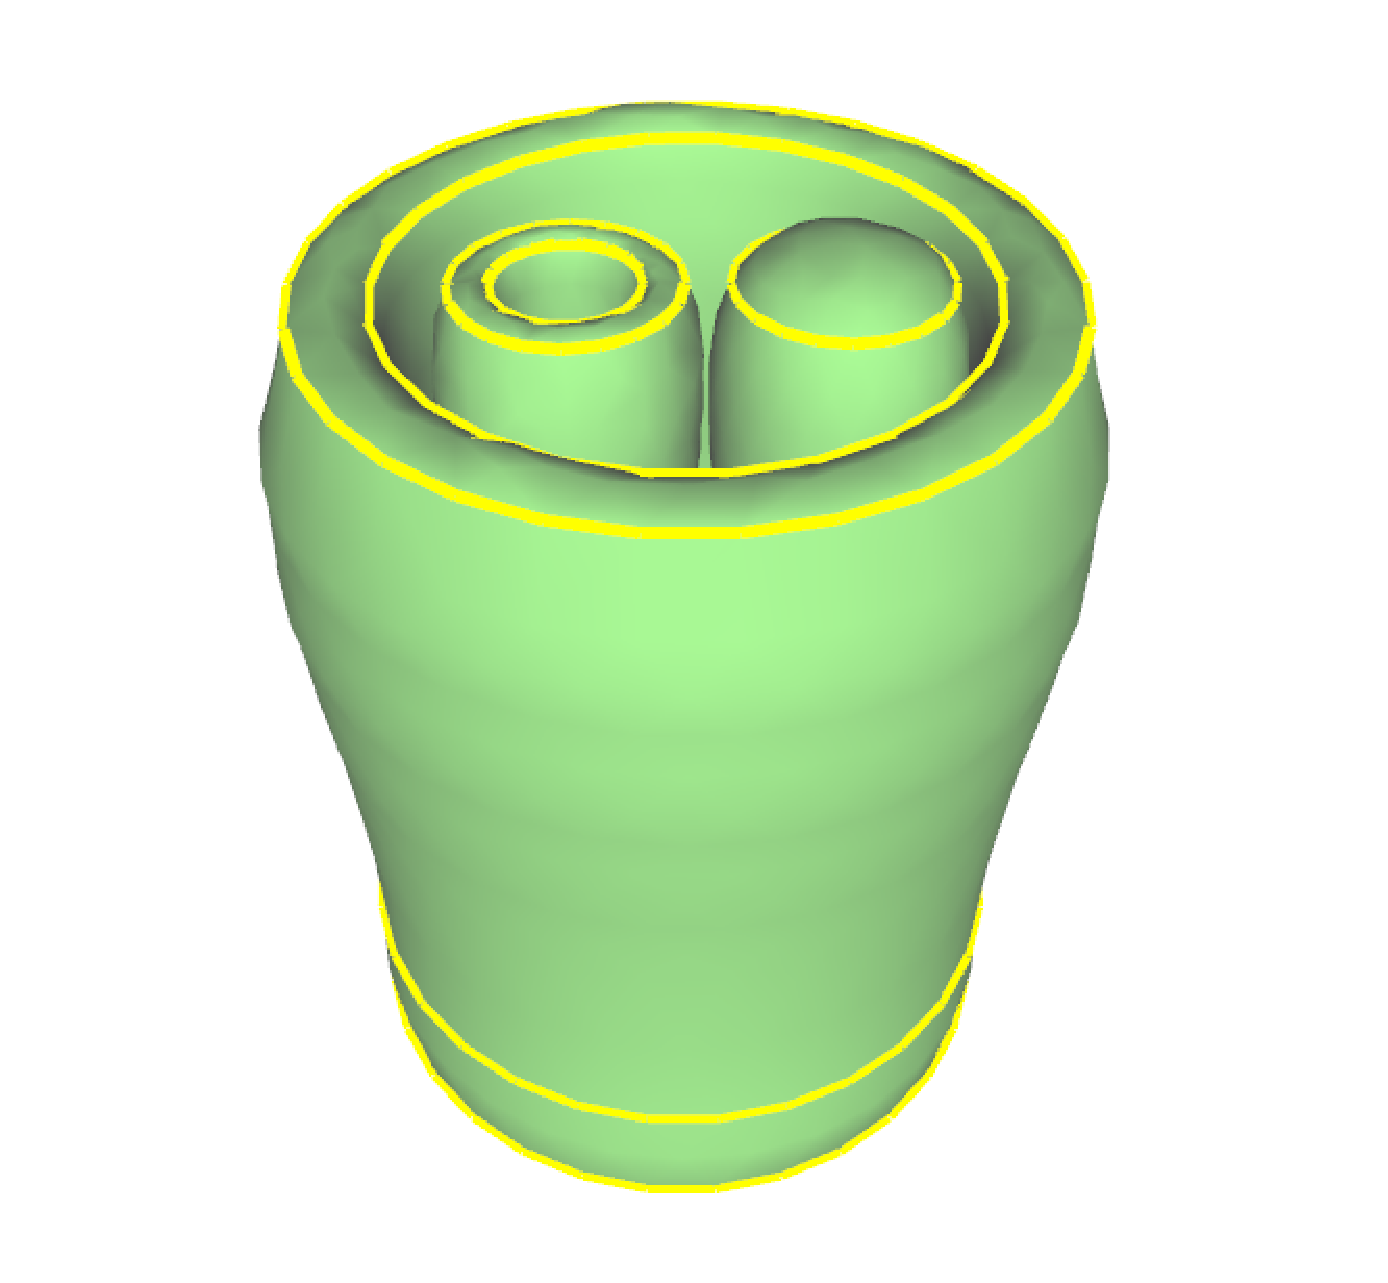
\includegraphics[scale=0.12]{figs/f3.rule2-2.eps}
    \end{minipage}}
  \caption{An example for rule~\ref{rule:2}. (a) The user sketched cross sections. Containing relationship exists among multiple cross sections on the blue plane; (b) The generated model.}
  \label{fig:rule2} %% label for entire figure
\end{figure}

Rule~\ref{rule:3} just does not allow self-intersection of one
curve or intersection between any two curves on the same plane since
it unlikely happens for the cross section contour of an object to
have intersection.

Rule~\ref{rule:4} can also be stated in another way that the
intersection points between the two curves and the intersection line
of the two planes must be be in the same positions. This rule
actually conforms to our common understanding of appearance of a 3D
object. It is difficult to imagine what the shape of the model will
be if the two sets $\{V_{S_1P_2}\}$ and $\{V_{S_2P_1}\}$ are not
same. However in practice, it is almost impossible for the users to
draw two exactly intersected curves manually. So after the curve
$S_1$ is drawn, we highlight the point set $\{V_{S_1P_2}\}$ to help
the users carefully draw the curve $S_2$ to make it pass through
$\{V_{S_1P_2}\}$ (see Figure~\ref{fig:csinters:a}). Then we perform
a curve deformation procedure, which is explained below, to
automatically sew the two curves up before constructing the surface.

For simplicity, let us assume there are two elements  in set
$\{V_{S_1P_2}\}$, which implies two curves $S_1$ and $S_2$ should
intersect at two points. So the goal here is to deform the two
curves, making them intersect at two points and meanwhile preserve
their original shape as much as possible.

First we calculate the intersection point set  $\{V_{S_1P_2}\}$
between $S_1$ and $P_2$, and $\{V_{S_2P_1}\}$ between $S_2$ and
$P_1$. Then we find two pairs of different closest points, in each
pair the two points are from $\{V_{S_1P_2}\}$ and $\{V_{S_2P_1}\}$
respectively. The midpoints $V_{m1}$ and $V_{m2}$ of these two pairs
are treated as the new positions of the handle points. Two handle
points on each curve can then be chosen as the points closest to
$V_{m1}$ and $V_{m2}$ respectively. Next a range of points near the
handles are to be moved with them and we need to compute their new
positions. So we could perform the Laplacian deformation algorithm
to the two curves to deform them. Since the two curves are both
planar, it can be further simplified into a 2D deformation problem
which can be precisely solved~\cite{ESA07}.

\begin{figure} [htbp]
  \centering
  \subfigure[]{
    \centering
    \label{fig:curvemerge:a} %% label for first subfigure
    \begin{minipage}[b]{0.25\textwidth}
      \centering
      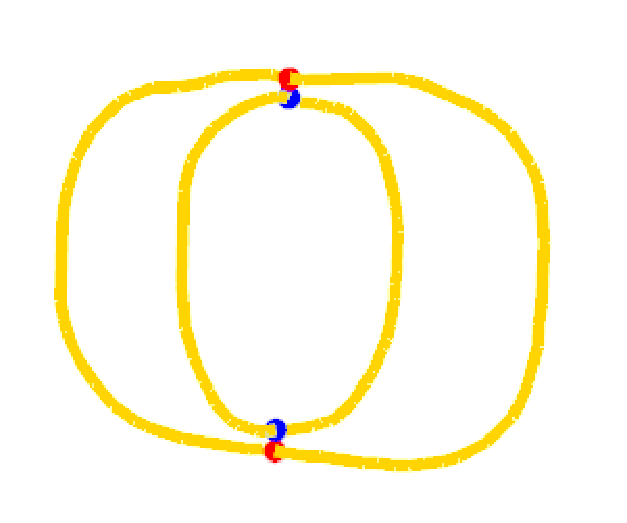
\includegraphics[scale=0.35]{figs/f3.CurveMerge1.eps}
    \end{minipage}}
  \subfigure[]{
    \centering
    \label{fig:curvemerge:b}
    \begin{minipage}[b]{0.25\textwidth}
      \centering
      
\includegraphics[scale=0.35]{figs/f3.CurveMerge2.eps}
    \end{minipage}}
  \subfigure[]{
    \centering
    \label{fig:curvemerge:c}
    \begin{minipage}[b]{0.25\textwidth}
      \centering
      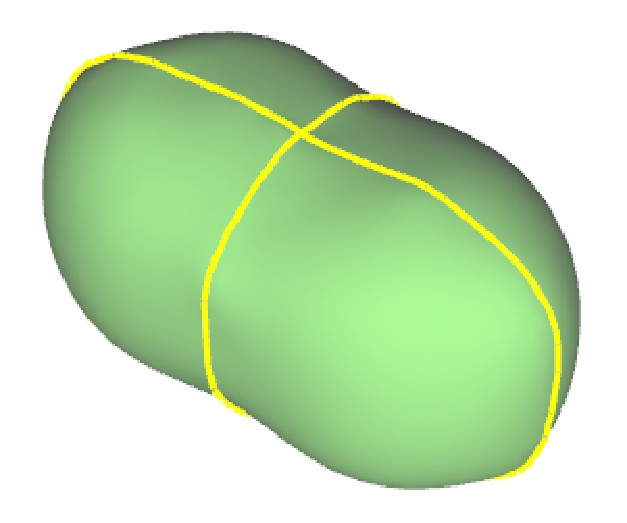
\includegraphics[scale=0.35]{figs/f3.CurveMerge3.eps}
    \end{minipage}}
  \caption{Curve sewing. (a) Two curves lie on two orthogonal planes. The colored points denote the intersection points between a curve and a plane that another curve lies on. (b) Deform the two curves so that they intersect at two points. (c) Generate a mesh that takes the two curves as contours.}
  \label{fig:curvemerge} %% label for entire figure
\end{figure}

It can be seen from Figure~\ref{fig:curvemerge} that  during the
deformation process, no extra discontinuity will be caused at the
intersection part of each curve and the deformed curves keep their
original shapes very well, thus preserving the original
characteristics of the user input strokes.

The above mentioned steps are for the simple two-contour  case. For
multiple contours, we just need to deal with them one by one to make
them accord with the rules we defined.

The curve sewing process can handle inconsistent cross sections
automatically, which meets the requirement on the user interface
design that the system should constructively suggest a solution to
help users to recover from errors~\cite{MN90}. By proposing these
rules and strategies, our sketching interface will become more
natural and intelligent to the user.

After all these processes, we are finally ready to construct  the
mesh model. The details on the progressive reconstruction algorithm
will be presented in Chapter~\ref{ch:orthsurf}.


\subsection{Reference plane calculation}
\label{ch3:sec:algo:refplane}

As mentioned in Section~\ref{ch3:sec:ui:sculpt:deform}, we provide
the users reference planes for drawing the deformed shape of the
handle curve in the deformation function. A key problem here is how
to generate the base plane which has a suitable position and
direction, as the projection plane could be easily calculated after
the base plane is confirmed.

Our basic idea is to let the base plane go through as many points of
the handle curve as possible. For this purpose, we compute the least
squares plane that fits the points. Assume the plane equation is

\begin{equation}
\label{eq:planefunc}
    Ax+By+Cz+D=0,
\end{equation}
where $A$, $B$, $C$ and $D$ are the unknown parameters to be determined,
and we let $A^2+B^2+C^2=1$, which means
$N = [\begin{array}{*{20}c} A & B & C \end{array}]$ is the unit normal
vector of the plane. Then our task is to find the plane that minimizes
the following objective function

\begin{eqnarray}
\label{eq:planeobjnoZ0}
    f(A,B,C,D) &=& \sum\limits_{i \in HC}
    {\frac {(Ax_i+By_i+Cz_i+D)^2}{A^2+B^2+C^2}},\nonumber\\
    &=& \sum\limits_{i \in HC} {(Ax_i+By_i+Cz_i+D)^2},
\end{eqnarray}
where $i \in HC$  means $p_i=(x_i,y_i,z_i)$ is a point on the handle curve.

%%%introduce the solving of this optimization problem
To solve this optimization problem, we used the method proposed
in~\cite{SWMB59}. First, we set the partial derivative of
$f(A,B,C,D)$ w.r.t. $D$ equal to zero and get:

\begin{eqnarray}
\label{eq:planeobjPartD}
    \sum\limits_{i \in HC} {(Ax_i+By_i+Cz_i+D)} = 0\nonumber\\
    D = -(Ax_c + By_c + Cz_c),
\end{eqnarray}
where $(x_c, y_c, z_c)$ represents the centroid of all the
input points on the handle curve. Then we substitute $D$ back
to Eq.~\ref{eq:planeobjnoZ0}, and the function to minimize can
be written as:

\begin{eqnarray}
\label{eq:planeobjnew}
    f(A,B,C) &=& \sum\limits_{i \in HC} {(A(x_i-x_c)+B(y_i-y_c)+C(z_i-z_c))^2}\nonumber\\
    &=& (NM^T)(MN^T)\nonumber\\
    &=& N (M^TM) N^T,
\end{eqnarray}
where $N = [\begin{array}{*{20}c} A & B & C \end{array}]$
is the unit normal vector of the plane we have mentioned
and $M$ is the matrix defined as:

\begin{equation*}
\begin{bmatrix}
x_1-x_c & y_1-y_c & z_1-z_c\\[-1em]
x_2-x_c & y_2-y_c & z_2-z_c\\[-1em]
\cdot & \cdot & \cdot\\[-1em]
\cdot & \cdot & \cdot\\[-1em]
\cdot & \cdot & \cdot\\[-1em]
x_n-x_c & y_n-y_c & z_n-z_c
\end{bmatrix},
\end{equation*}
assuming there are $n$ points on the handle curve. Next, $f(A,B,C)$
can be minimized by computing the singular value decomposition
of $M=USV^T$ and letting $P$ equal to the third column
of $V$. To this end, the parameters of the optimal plane in
Eq.~\ref{eq:planefunc} can be obtained. It can be seen that
the calculated plane will interpolate the centroid of the
input points and its normal vector is the singular vector
of $M$ corresponding to its smallest singular value.

%%%


The above method just gives a suggestive orientation of the base
plane. If the user is not satisfied, he/she can rotate the plane by
a proper angle. The axis of the rotation is the line connecting the
projection of the first handle point onto the initial computed plane
to that of the last point. The calculation of the reference plane
for extrusion process is the same as this.

After the reference planes are constructed, the user can sketch the
new shape and position of the handle curve. If the user intends to
draw a non-planar curve by sketching the shadow of the base plane
curve on the projection plane, we use the algorithm proposed
in~\cite{CMZHB99} to combine the two planar curves to generate a
spatial one.

Once the ROI vertices, the handle curve and its new shape are
confirmed, we complete the deformation by employing a flexible mesh
deformation algorithm, which will be presented in
Chapter~\ref{ch:flexdeformation}.


%-------------------------------------------------------------------------
\section{Results and discussions}
\label{ch3:sec:result}

\begin{figure*} [htbp]
  \centering
  \subfigure[Mushroom]{
    \centering
    \label{fig:mushroom} %% label for first subfigure
    \begin{minipage}[b]{\textwidth}
      \centering
      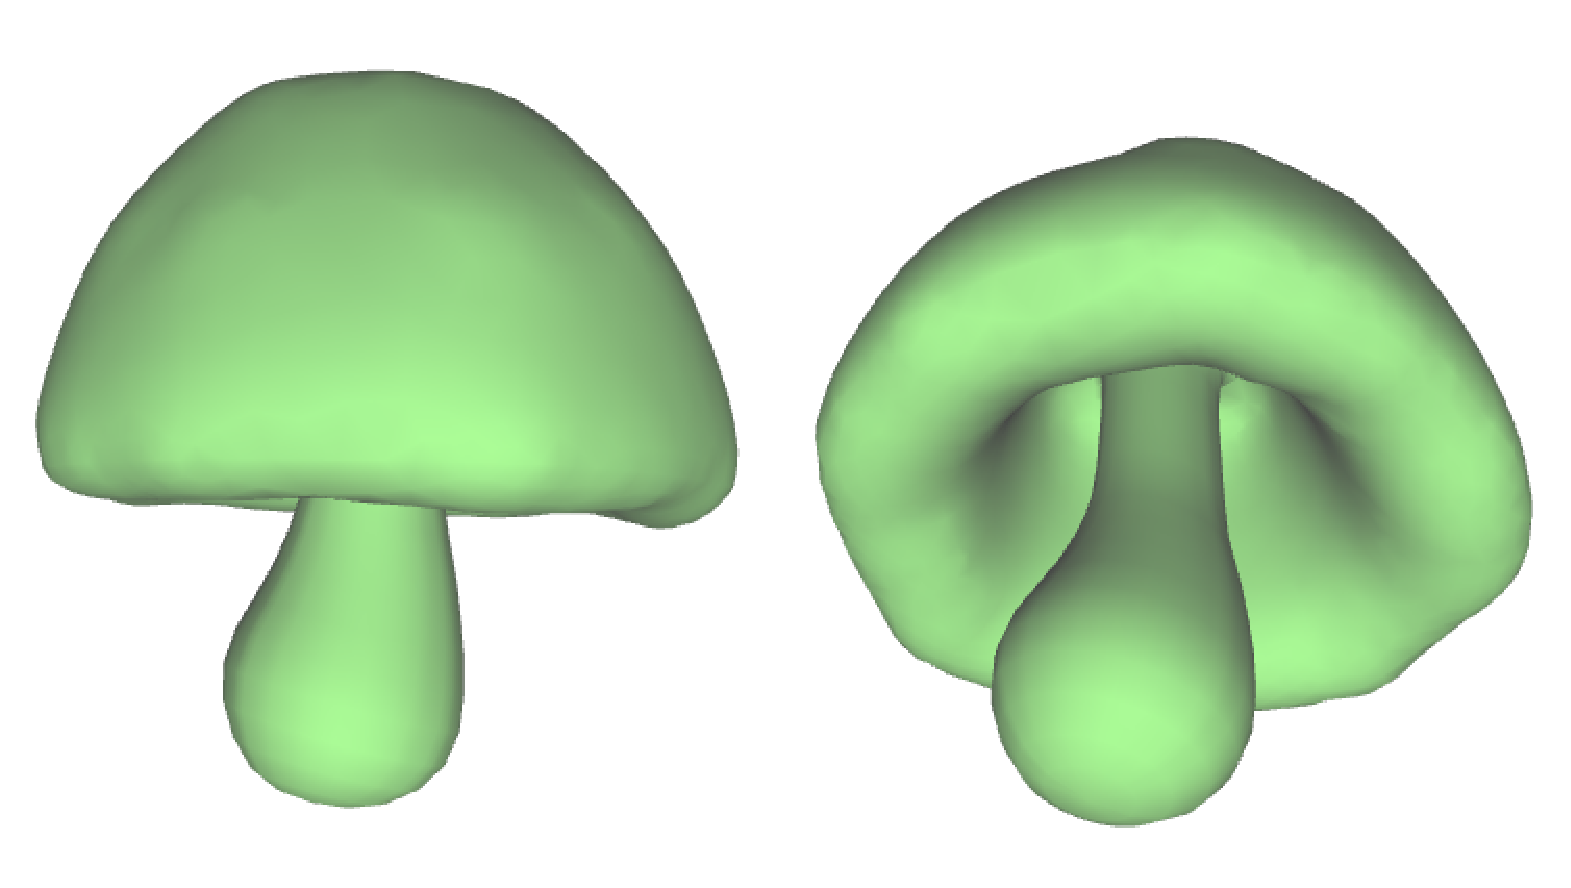
\includegraphics[scale=0.1]{figs/f3.mushroom.eps}%0.09
    \end{minipage}}
  \subfigure[Handicraft]{
    \centering
    \label{fig:6hole} %% label for first subfigure
    \begin{minipage}[b]{\textwidth}
      \centering
      \includegraphics[scale=0.1]{figs/f3.6hole.eps}
    \end{minipage}}
  \subfigure[Car]{
    \centering
    \label{fig:car} %% label for first subfigure
    \begin{minipage}[b]{\textwidth}
      \centering
      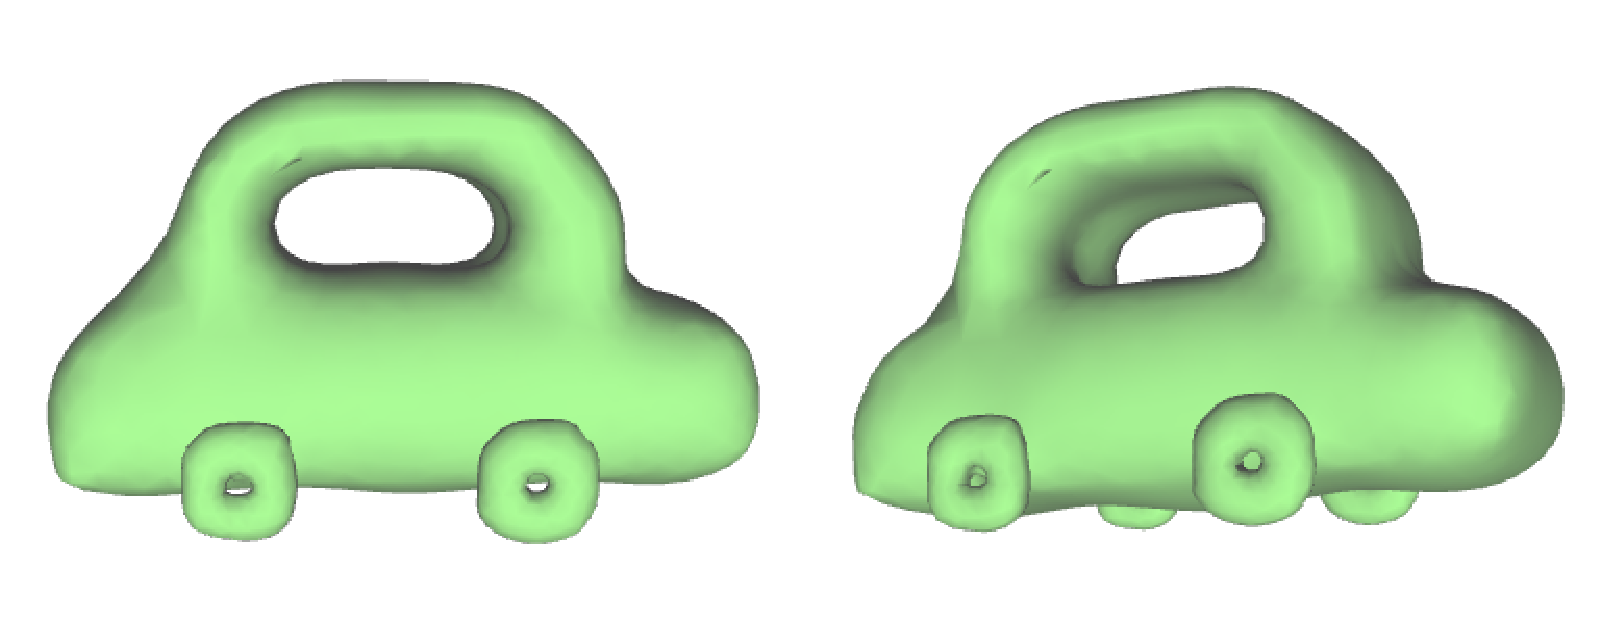
\includegraphics[scale=0.1]{figs/f3.car.eps}
    \end{minipage}}
  \subfigure[Censer]{
    \centering
    \label{fig:censer} %% label for first subfigure
    \begin{minipage}[b]{\textwidth}
      \centering
      \includegraphics[scale=0.1]{figs/f3.censer.eps}
    \end{minipage}}
  \subfigure[Bicycle]{
    \centering
    \label{fig:bike} %% label for first subfigure
    \begin{minipage}[b]{\textwidth}
      \centering
      \includegraphics[scale=0.1]{figs/f3.bike.eps}
    \end{minipage}}
  \subfigure[Sculpture]{
    \centering
    \label{fig:sculpture} %% label for first subfigure
    \begin{minipage}[b]{\textwidth}
      \centering
      \includegraphics[scale=0.1]{figs/f3.sculpture.eps}
    \end{minipage}}
  \caption{The sketching of some models using our system.}
  \label{fig:models:sketch} %% label for entire figure
\end{figure*}

\begin{figure*} [htbp]
  \subfigure[Cup]{
    \centering
    \label{fig:cup} %% label for first subfigure
    \begin{minipage}[b]{\textwidth}
      \centering
      \includegraphics[scale=0.12]{figs/f3.cup.eps}
    \end{minipage}}
  \subfigure[Rabbit]{
    \centering
    \label{fig:rabbit} %% label for first subfigure
    \begin{minipage}[b]{\textwidth}
      \centering
      \includegraphics[scale=0.12]{figs/f3.rabbit.eps}
    \end{minipage}}
  \subfigure[Chair]{
    \centering
    \label{fig:chair} %% label for first subfigure
    \begin{minipage}[b]{\textwidth}
      \centering
      \includegraphics[scale=0.12]{figs/f3.chair.eps}
    \end{minipage}}
  \caption{The sketching and sculpting of some models using our system.}
  \label{fig:models:combine} %% label for entire figure
\end{figure*}

%basic information
Our current implementation of this sketch-based modeling system was
written  in C++ on the Windows platform. We tested our system on an
machine with Dual Core Intel Xeon 2.27GHz CPU and 2G RAM. Our
experiments show that both the surface reconstruction and other
sculpting functions run in interactive rates. This indeed meets the
user's requirement on a sketch-based modeling system.

%computation complexity and cost
It is observed that even if multiple cross section curves are
sketched initially, the constructed mesh is not quite dense, and
the number of vertices will be no more a few thousands after
iterative editing operations. This enables us to consider more about
the modeling effect and quality of the mesh other than the running
time. Meanwhile, the modeling algorithms we developed also ensure
that computation will be completed in real time, which can be
introduced in the next chapters.

%For the surface reconstruction in our sketching tool, the shape built from each cross section is just simple cylinders, so the CSG computation is relatively simple and little numerical issues are involved. It is observed that even if multiple cross section curves are sketched initially, the constructed mesh is not quite dense, and the number of vertices will be no more a few thousands after iterative editing operations. This enables us to consider more about the modeling effect and quality of the mesh other than the running time.

%user study
We have conducted an informal user study to test our system.  We
trained the novice users for approximately 20 minutes and let them
create models with freeform shapes. We found that most users tend to
use the sketching tool to iteratively sketch and construct the 3D
models in most of the time and just take the sculpting tools to do
some detail modifications, although there are a few who prefer to
build a model by sculpting it from a rough shape (see
Figure~\ref{fig:chair}). This is consistent with the introduction
in~\cite{CIW08} that the sketching technique is more familiar to
public than sculpting which requires tedious manual work. Some
results produced with either the sketching tool or the combination
of the two tools are shown in Figure~\ref{fig:models:sketch} and
Figure~\ref{fig:models:combine}. All of these models are produced in
less than 30 minutes.

We learned from the feedback that with help of the reference planes,
the users can get a direct \lq\lq{touch}\rq\rq of the 3D space and
they only need to focus on the sketching of the curves for defining
the shape of the 3D model. The reference shape together with the
existing sketches let them get a clear mind of the 3D model in each
design stage and also give hints for the next sketches. Some issues
exist in other systems such as difficulties on confirming the
position and orientation of the 3D curves corresponding to the 2D
sketches, the imagination of the sketched 3D shape and so on can be
avoided. Although the users do not adapt to the stroke rules quite
well initially, they get used to it gradually with the help of
various hints in our system during the studying process and find it
quite helpful for eliminating perception ambiguities eventually.




%%-------------------------------------------------------------------------
%\section{Conclusions}
%\label{ch3:sec:concl}
%
%We have described a novel sketching interface for creating and editing 3D models. The main contributions are:
%
%\begin{itemize}
%   \item We propose a progressive modeling approach to enhance the creation function in sketch-based modeling, by allowing the user to create a 3D model through iterative sketches, taking both the existing sketches and the shape in each design stage as references. The user can thus get fully aware of the 3D shape which changes naturally with each new sketch and unexpected result can be avoided. Supporting surface reconstruction algorithm for this approach is developed to produce natural shape changes and models with single connected components.
%   \item We propose the strategy of using auxiliary planes as references for creation, deformation and other editing operations in the sketching interface. Reference planes help make the sketch-based modeling process intuitive and easy to use.
%   \item We propose stroke rules for regularizing and interpreting the user input sketches. These rules consider both the semantic meaning of the sketched strokes and human psychology.
%\end{itemize}
%
%In future, the surface reconstruction algorithm for the progressive modeling can be further accelerated using parallel computing or other techniques, since the computation within each zone is totally independent. In addition, we will explore the use of more types of geometry objects as references to assist sketch-based interface and modeling.
